\documentclass[lang=en,color=blue,mode=fancy,titlestyle=hang]{elegantbook}

% ---- Title Information ----
\title{Introduction to Convex Optimization}
\author{Lancet Ross}
\date{Jul 22, 2026}
\version{1.0}
\extrainfo{``You don't need a starting point, you don't need to babysit the algorithm. --- Stephen Boyd''}
\cover{cover.pdf}

% ---- Additional Packages ----
\usepackage{algorithm}
\usepackage{algpseudocode}
\usepackage{float}
\usepackage{subcaption}

% ---- Math Operators ----
\DeclareMathOperator*{\argmin}{arg\,min}

\begin{document}

% ---- Title Page ----
\maketitle

\frontmatter
\tableofcontents

\chapter*{Preface}
\addcontentsline{toc}{chapter}{Preface}

When talking about optimization, we usually think of the optimization problem as a black box.
We give it an input, and it gives us an output. But in reality, it is not. Optimization is a
process of searching for the best solution in a feasible set. In this process, we need to
consider the properties of the feasible set and the objective function. If we can find a way to
exploit these properties, we can design more efficient algorithms.

This tutorial is designed to introduce the basic concepts of convex optimization, from the
mathematical foundations to practical algorithms. It is intended for readers who have some
background in linear algebra — you should know what a matrix is, what eigenvalues are, and
how to multiply matrices without breaking a sweat. If these terms sound unfamiliar, you may
want to read my linear algebra tutorial first. Some familiarity with MATLAB is also helpful
but not required; the code examples are simple enough to translate to Python or Julia.

The tutorial mainly follows Prof.\ Ling Qing's open course at USTC. His lectures are clear,
intuitive, and full of geometric insight — I cannot recommend them enough. You can find the full
playlist on Bilibili. For deeper study, Stephen Boyd's textbook \textit{Convex Optimization}
remains the standard reference, though it demands more mathematical maturity than this tutorial
assumes. I have added several chapters on algorithms that go beyond both Prof.\ Ling's course
and Boyd's book, covering modern methods that you will actually encounter in research and practice.

\subsection*{How this tutorial is organized}

\textbf{Chapters 1–2} cover the geometry of convex sets and convex functions. These are the
building blocks — every result later in the book traces back to definitions you will see here.

\textbf{Chapters 3–4} introduce convex optimization problems and duality. The Karush–Kuhn–Tucker
(KKT) conditions are the centerpiece: they tell you when a point is truly optimal, and they
are the theoretical backbone of almost every algorithm that follows.

\textbf{Chapters 5–7} shift from theory to computation. We start with gradient descent —
the simplest possible method — and gradually work our way up through Newton's method,
equality-constrained minimization, ADMM, accelerated first-order methods (FGP, FISTA,
Forward-Backward Splitting), and second-order methods for nonlinear least squares
(Gauss–Newton, Levenberg–Marquardt, BFGS).

Unlike most convex optimization textbooks that either get lost in excessive mathematical rigor
or jump straight to theory without showing the algorithmic landscape, this tutorial tries to strike
a balance. Every algorithm is accompanied by intuition, convergence analysis, and MATLAB
code. The proofs are included where they illuminate the idea; they are omitted or sketched
where they become tedious.

\subsection*{How to read this tutorial}

One final piece of advice: do not just read the formulas. Write them down. Implement the
algorithms on small synthetic problems — a random quadratic in $\mathbb{R}^{10}$, a simple
LASSO problem, a tiny image inpainting task. Change the parameters and see what happens.
Plot the convergence curves. Watch gradient descent zigzag when the condition number is bad,
then watch Newton's method take two steps and stop. Optimization is a field where intuition
is built through experimentation, not through passive reading. If you do that, this tutorial has
served its purpose.

I am grateful to Prof.\ Ling Qing for making his lectures freely available, and to the open-source
community behind \LaTeX, the ElegantBook template, and the countless tools that made writing
this tutorial a pleasure rather than a chore. Any mistakes that remain are mine alone.

Now I think it is time to start.

\begin{flushright}
  Lancet Ross\\
  July 22, 2026
\end{flushright}

\mainmatter

\chapter{Convex Sets}
\section{Affine and convex sets}
\subsection{Affine sets}
A set C is affine if the line through any 2 distinct points in C lies in C. In other words,
C contains all linear combinations of its points, provided the coefficients sum to 1.

If C is an affine set, and $x_0 \in C$, then we call the new affine set
\[
V = C - x_0 = \{x - x_0 \;|\; x \in C\}
\]
is a subspace related to $C$. Suppose $v_1, v_2 \in V$, then for any
$\alpha, \beta \in \mathbb{R}$, we have
\[
\alpha v_1 + \beta v_2 \in V.
\]
This is because
\[
\alpha v_1 + \beta v_2 = \alpha (v_1 + x_0) + \beta (v_2 + x_0) + (1 - \alpha - \beta)x_0 \in C.
\]

Also, a subspace must contains the zero vector. It's obvious that $0 \in V$ since
\[
0 = 0 \cdot v_1 + 0 \cdot v_2 \in V.
\]

Next, here we give an example to describe the relationship between affine sets and linear
algebra: The solution of linear equations is an affine set.

Here is the math expression of linear equations:
\[
C = \{x \in \mathbb{R}^n \;|\; Ax = b\}
\]

We notice that $Ax_0 = b$, so shifting $x_0$ gives us the subspace
\[
V = C - x_0 = \{x - x_0 \;|\; A(x - x_0) = 0\} = \{y \in \mathbb{R}^n \;|\; Ay = 0\}.
\]

See what? $V$ is the nullspace of $A$.

If there is an arbitrary set $C$, how can we find the smallest affine set containing it?
We need to introduce the concept of the affine hull of $C$, denoted by $\textbf{aff} \; C$.
And denoted $\textbf{aff} \; C$:
\[
\textbf{aff} \; C = \left\{\sum_{i=1}^{k} \theta_i x_i \;|\; x_i \in C, \; \sum_{i=1}^{k} \theta_i = 1, \theta_i \in \mathbb{R}, k \in \mathbb{N}\right\}.
\]

\subsection{Convex sets}
A set C is convex if the line segment between any 2 points in C lies in C. In other words,
for any $x_1, x_2 \in C$ and $\theta \in [0, 1]$, we have
\[
\theta x_1 + (1 - \theta) x_2 \in C.
\]

Also, a convex combination of points in $C$ is any point of the form
\[
\sum_{i=1}^{k} \theta_i x_i \quad \text{where} \quad x_i \in C, \; \sum_{i=1}^{k} \theta_i = 1, \; \theta_i \in [0, 1].
\]

Now we can expand the definition of convex sets. A set $C$ is convex if, for any elements
in $C$, those convex combinations also lie in $C$.

As with affine sets, we can define the convex hull of an arbitrary set $C$, denoted by
\[
\textbf{conv} \; C = \left\{\sum_{i=1}^{k} \theta_i x_i \;|\; x_i \in C, \; \sum_{i=1}^{k} \theta_i = 1, \; \theta_i \geq 0, \; k \in \mathbb{N}\right\}.
\]

\begin{figure}[H]
  \centering
  \begin{subfigure}[t]{0.49\textwidth}
    \centering
    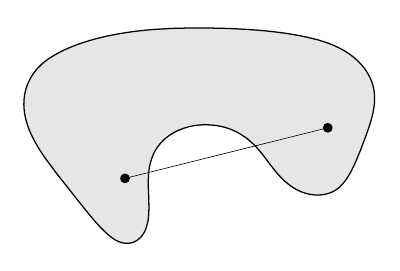
\includegraphics[width=\textwidth]{assets/1 Convex sets/1.1 Affine and convex sets/convex set.png}
    \caption{Convex Set}
  \end{subfigure}
  \hfill
  \begin{subfigure}[t]{0.49\textwidth}
    \centering
    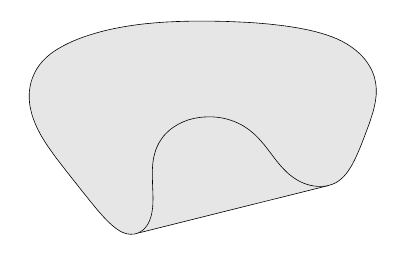
\includegraphics[width=\textwidth]{assets/1 Convex sets/1.1 Affine and convex sets/convex hull.png}
    \caption{Convex Hull}
  \end{subfigure}
\end{figure}

\subsection{Convex cones}

A set $C$ is a cone if, for any $x \in C$ and $\alpha \geq 0$, we have $\alpha x \in C$.

A set $C$ is a convex cone if, for any $x_1, x_2 \in C$ and $\theta_1, \theta_2 \geq 0$,
we have $\theta_1 x_1 + \theta_2 x_2 \in C$.

Similar to things above, we can define the conic hull of an arbitrary set $C$, denoted by
\[
\textbf{cone} \; C = \left\{\sum_{i=1}^{k} \theta_i x_i \;|\; x_i \in C, \; \theta_i \geq 0, \; \theta_i \in \mathbb{R}, k \in \mathbb{N}\right\},
\]
among this, $\sum_{i=1}^{k} \theta_i x_i$ is a conic combination of points in $C$.

\begin{figure}[H]
  \centering
  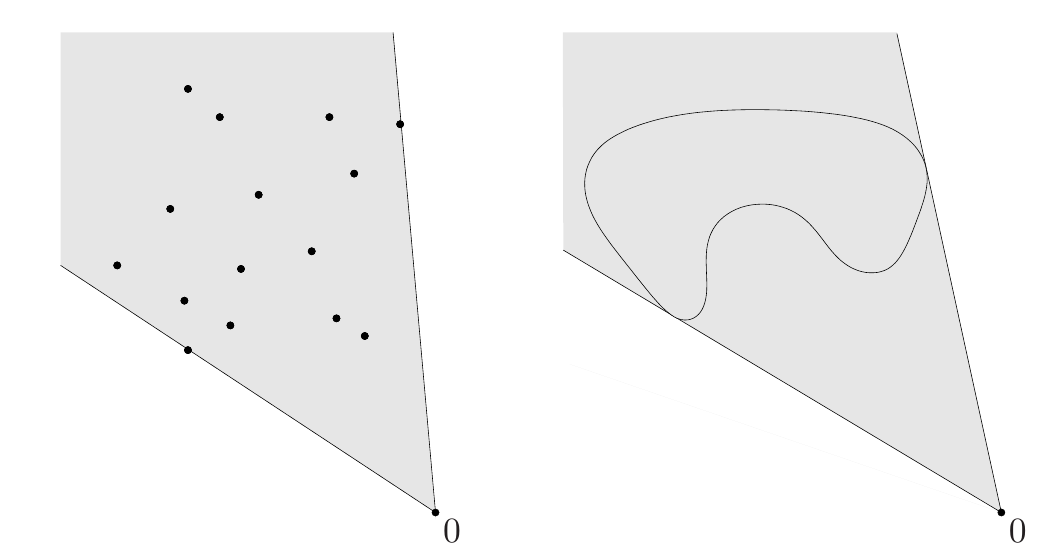
\includegraphics[width=\textwidth]{assets/1 Convex sets/1.1 Affine and convex sets/conic hull.png}
  \caption{Conic Hull}
\end{figure}

\section{Some important examples}
\subsection{Scattered situations}

\begin{itemize}
  \item A single point set $\{x_0\}$ is convex and affine, only if $x_0 = 0$ it's
  a convex cone.
  \item $\emptyset$, $\mathbb{R}^n$ and subspaces (in the sense of linear algebra)
  is convex, affine and a convex cone.
  \item A straight line is affine, convex and not a convex cone unless it passes
  through the origin.
  \item A line segment is convex, but not affine unless it reduces to a point at
  the origin.
  \item A ray which has the form $\{x_0 + \theta v \;|\; \theta \geq 0\}$ and
  $v \neq 0$ is convex, not affine, and not a convex cone only when $x_0 = 0$.
\end{itemize}

\subsection{Hyperplanes and halfspaces}
A hyperplane in $\mathbb{R}^n$ is a set of the form
\[
 \{x \;|\; a^T x = b\},
\]
where $a \neq 0$, $a \in \mathbb{R}^n$ and $b \in \mathbb{R}$.

A hyperplane divides $\mathbb{R}^n$ into two halfspaces:
\[
H^+ = \{x \in \mathbb{R}^n \;|\; a^T x \geq b\}
\]
and
\[
H^- = \{x \in \mathbb{R}^n \;|\; a^T x \leq b\}.
\]

\begin{figure}[H]
  \centering
  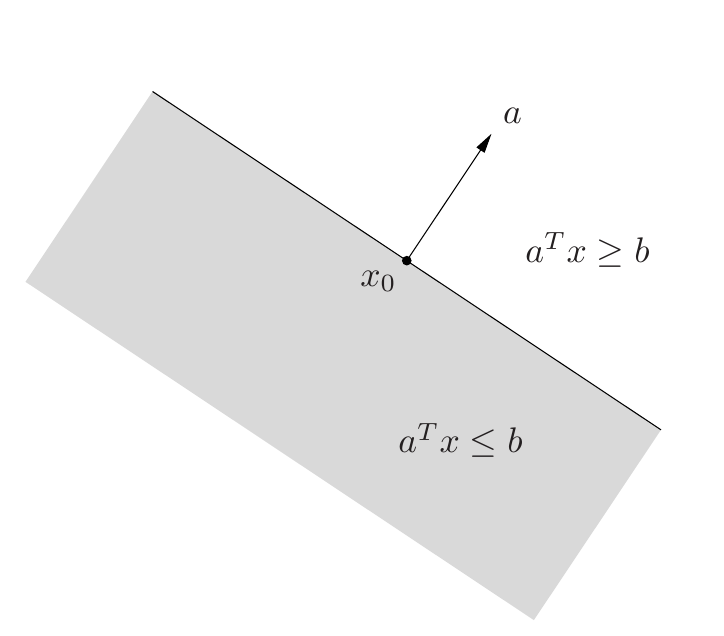
\includegraphics[width=0.7\textwidth]{assets/1 Convex sets/1.2 Some important examples/hyperplane and halfspace.png}
  \caption{Hyperplane and Halfspace}
\end{figure}

Hyperplane is affine, convex and not a convex cone unless it passes through the origin.

Halfspaces are convex, but not affine. They are convex cones only when $b = 0$.

\subsection{Euclidean balls and ellipsoids}

A Euclidean ball in $\mathbb{R}^n$ is a set of the form
\[
B(x_c, r) = \{x \;|\; (x - x_c)^{T} (x - x_c) \leq r^2\}
\]
where $x_c$ is the center and $r > 0$ is the radius. It's convex, not affine, and not
a convex cone.

Ellipsoids are sets of the form
\[
\mathcal{E} = \{x \;|\; (x - x_c)^{T} P^{-1} (x - x_c) \leq 1\},
\]
where $x_c$ is the center and $P = r^{2}I_r$ is a positive definite matrix. Its singular
value defines the semimajor axis lengths of the ellipsoid.

It's clear that ellipsoid is convex, not affine, and not a convex cone.

\subsection{Polyhedra and simplices}

A polyhedron in $\mathbb{R}^n$ is a set defined by a finite number of linear inequalities:
\[
\mathcal{P} =
\left\{
x \;\middle|\;
\begin{aligned}
  &a_j^T x \le b_j, \quad j = 1,\ldots,m \\
  &c_j^T x = d_j, \quad j = 1,\ldots,p
\end{aligned}
\right\}.
\]

It is convex, not affine, and not a convex cone unless all the equalities pass through
the origin.

What's more, a polyhedron can be represented as the intersection of a finite number
of halfspaces.

\begin{figure}[H]
  \centering
  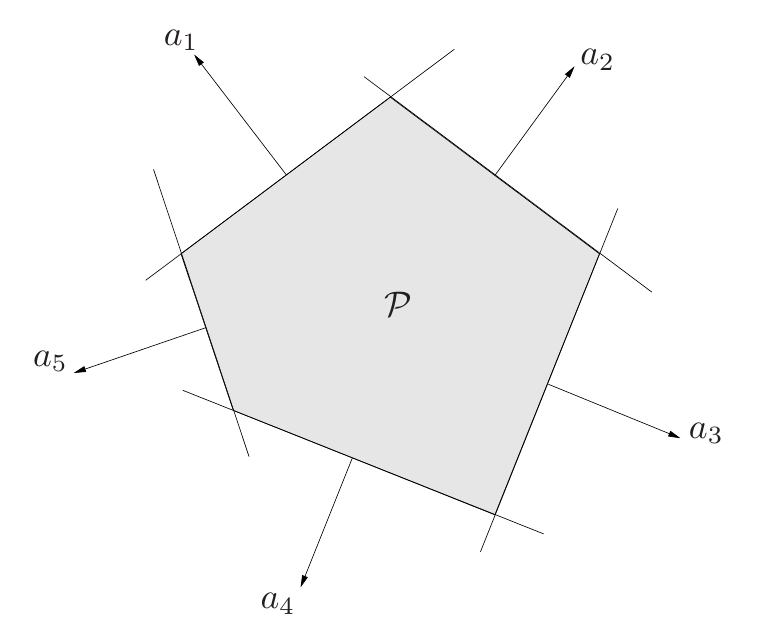
\includegraphics[width=0.7\textwidth]{assets/1 Convex sets/1.2 Some important examples/polyhedron.png}
  \caption{Polyhedron}
\end{figure}

Suppose $k + 1$ points $x_0, x_1, \ldots, x_k$ in $\mathbb{R}^n$ are affinely independent,
which means that the set $\{x_1 - x_0, x_2 - x_0, \ldots, x_k - x_0\}$ is linearly independent.
The simplex formed by these points is
\[
C = \textbf{conv} \{x_0, x_1, \ldots, x_k\}
\]

According to the definition of linear combinations, you can only find $n + 1$ affinely
independent points in $\mathbb{R}^n$ to form a simplex.

And here is an important property that simplices must be polyhedra.

It's not always easy to see, before we start, there is a linear algebra problem to solve,
why a column full rank matrix $B$ can be left multiplied by a invertible squared matrix $A$ and
get $[I \; 0]^T$.

We can assume
\[
A = \begin{bmatrix} A1 \\ A2 \end{bmatrix}
\]
which $A1$ is the pseudo-inverse of $B$ and $A2$ is in the left null space of $B$. Then we have
\[
A B = \begin{bmatrix} I \\ 0 \end{bmatrix}.
\]

After that we can start the proof.

Define
\begin{align*}
y &= [\theta_1 \theta_2 \ldots \theta_k]^T, \text{ where } y \geq 0 \text{ and } 1^{T}y = 1 \\
B &= [v_1 - v_0 \; v_2 - v_0 \; \ldots \; v_k - v_0]
\end{align*}

So we can rewrite $x \in C$ to
\begin{align*}
x &= \sum_{i=0}^{k} \theta_i v_i \\
  &= v_0 + \sum_{i=1}^{k} \theta_i (v_i - v_0) \\
  &= v_0 + B y,
\end{align*}
and left multiply $A$ to both sides:
\[
A x = A v_0 + A B y.
\]

Divide this equation to 2 parts:
\begin{align}
A_1x &= A_1 v_0 + y \\
A_2x &= A_2 v_0
\end{align}

Equation (1) can be rewritten as
\begin{align}
A_1x &\geq A_1 v_0 \\
1^{T}A_1x &\leq 1^{T}A_1 v_0 + 1
\end{align}

Now we use (2) (3) (4) to represent a simplex, this is just the definition of a polyhedra.

\subsection{The positive semidefinite matrices}

We use $S^n$ to denote the set of symmetric $n \times n$ matrices, $S^n_+$ to denote
the set of positive semidefinite matrices and $S^n_{++}$ to denote the set of positive
definite matrices:
\begin{align*}
S^n &= \{X \in \mathbb{R}^{n \times n} \;|\; X = X^{T}\} \\
S^n_+ &= \{X \in S^n \;|\; X \succeq 0\} \\
S^n_{++} &= \{X \in S^n \;|\; X \succ 0\}.
\end{align*}

$S^n_+$ is obviously a convex cone, but $S^n_{++}$ is not because $\theta_i$ can be zeros
leads to a positive semidefinite matrix.

However, they are all convex sets.

\section{Operations that preserve convexity}
\subsection{Intersection}
Convexity will be preserved under intersection that if $S_a$ is convex for every
$a \in \mathcal{A}$, then $\bigcap_{a \in \mathcal{A}} S_a$ is also convex. This can be
expanded to subspaces, affine sets and convex cones.

\subsection{Affine functions}
We call $f: \mathbb{R}^n \rightarrow \mathbb{R}^m$ an affine function if it can be expressed
in the form
\[
f(x) = Ax + b,
\]
where $A$ is a linear transformation and $b \in \mathbb{R}^m$ is a constant vector. 

There is a also different definition of affine function, they are equal:
\[
f(\lambda x_1 + (1 - \lambda) x_2) = \lambda f(x_1) + (1 - \lambda) f(x_2) \quad \text{for all } x_1, x_2 \in \mathbb{R}^n, \; \lambda \in \mathbb{R}.
\]

Affine functions preserve convexity, meaning that if $S$ is a convex set and $f$ is an affine
function, then the image of $S$ under $f$ is convex, or:
\[
f(S) = \{f(x) \;|\; x \in S\}.
\]

Also, if $f: \mathbb{R}^k \rightarrow \mathbb{R}^n$ is an affine function, the inverse image
of $S$ under $f$ is convex:
\[
f^{-1}(S) = \{x \;|\; f(x) \in S\}.
\]

I must point out that $f^{-1}(S)$ here is \textbf{not the inverse of the function $f$}.

There are some important examples of affine functions.

First is addition, $S_1 + S_2$ is convex if $S_1$ and $S_2$ are convex sets. We can define:
\[
S_1 \times S_2 = \{(x_1, x_2) \;|\; x_1 \in S_1, x_2 \in S_2\}.
\]
This is convex, and we define $f(x_1, x_2) = x_1 + x_2$. This obeys what we know above.

Second is that the solution set of the linear matrix inequality (LMI) is convex.

LMI is
\[
A(x) = x_1A_1 + x_2A_2 + \ldots + x_nA_n \preceq B, \text{ where } B, A_i \in \mathbb{S}^m \text{ and } x_i \in \mathbb{R},
\]
which $S^m$ is a symmetric matrix set. $A(x) \preceq B$ means that $B - A(x)$ is a positive
semidefinite matrix.

Assume affine function $f: \mathbb{R}^n \rightarrow \mathbb{S}^m$ is defined as
\[
f(x) = B - A(x).
\]

Then the original problem can be rewritten as
\[
f(x) \succeq 0.
\]

If there is a positive semidefinite matrix cone
\[
C = \{M \in \mathbb{S}^m \;|\; M \succeq 0\}
\]

Then we know
\[
f(x) \in C \Rightarrow x \in f^{-1}(C).
\]

And the inverse image is convex.

Third is that the ellipsoid. We have talked about it in 1.2.3, now give the proof.

Let $u = P^{-\frac12}(x - x_c)$ or $x = f(u) = P^{\frac12}u + x_c$, then we can change
the ball's definition:
\begin{align*}
\{u \;|\; \|u\|_2 \leq r\} &= \{x \;|\;\|P^{-\frac12}(x - x_c)\|_2 \leq r\} \\
&= \{x \;|\; (x - x_c)^TP^{-1}(x - x_c) \leq r^2\}
\end{align*}

\subsection{Perspective functions}


We define perspective function $P: \mathbb{R}^{n+1} \rightarrow \mathbb{R}^n$ with
$\textbf{dom } P = \mathbb{R}^n \times \mathbb{R}^{++}$ as $P(z, t) = \frac{z}{t}$,
where $\times$ here represents Cartesian Product.

If $C \subseteq \textbf{dom } P$ is a convex set, then the image
\[
P(C) = \{ P(x) \;|\; x \in C\}
\]
is still convex. This can be described as: a convex object, view through a pin-hole camera,
leave a convex image.

\begin{figure}[H]
  \centering
  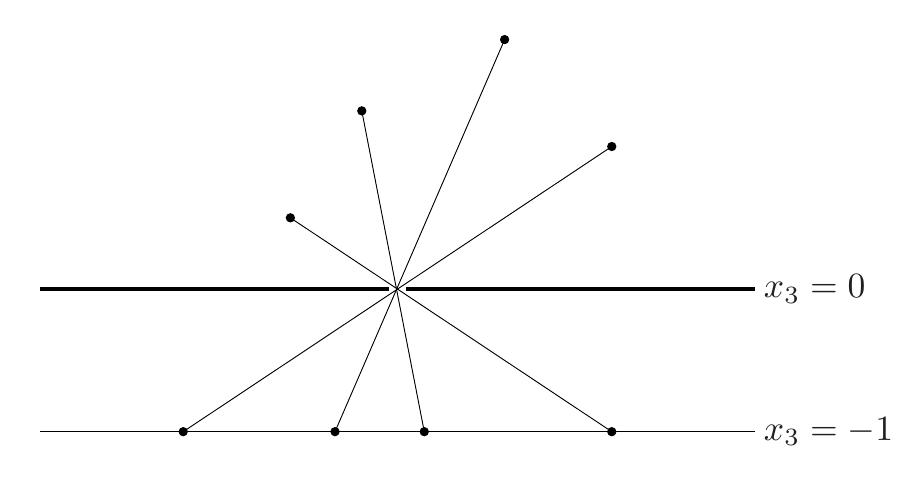
\includegraphics[width=0.7\textwidth]{assets/1 Convex sets/1.3 Operations that preverse convexity/perspective function.png}
  \caption{Perspective Function}
\end{figure}

A line segment through the pin-hole camera will project to a line segment in the image.

Suppose $x = (\tilde{x}, x_{n+1})$ and $y = (\tilde{y}, y_{n+1})$ are two points in the domain of $P$. The line segment connecting $x$ and $y$ can be expressed as:
\[
\{ \lambda x + (1 - \lambda) y \;|\; \lambda \in [0, 1]\}.
\]

Let the line segment go through the perspective function:
\begin{align*}
P(\lambda x + (1 - \lambda) y) &= \frac{\lambda \tilde{x} + (1 - \lambda) \tilde{y}}{\lambda x_{n+1} + (1 - \lambda) y_{n+1}} \\
&= \frac{\lambda x_{n+1}}{\lambda x_{n+1} + (1 - \lambda) y_{n+1}}\frac{\tilde{x}}{x_{n+1}} + \frac{(1 - \lambda) y_{n+1}}{\lambda x_{n+1} + (1 - \lambda) y_{n+1}}\frac{\tilde{y}}{y_{n+1}} \\
&= \mu P(x) + (1 - \mu) P(y),
\end{align*}

The inverse image of a convex set under a perspective function is also convex.
\[
P^{-1}(C) = \{ (x, t) \in \mathbb{R}^{n+1} \;|\; \frac{x}{t} \in C, \; t > 0\}
\]

Suppose $(x, t) \in P^{-1}(C)$, $(y, s) \in P^{-1}(C)$ and $\theta \in [0, 1]$. Then we have:
\begin{align*}
\theta x + (1 - \theta) y \in P^{-1}(C) &\Rightarrow \frac{\theta x + (1 - \theta) y}{\theta t + (1 - \theta) s} \in C. \\
&\Rightarrow \mu(\frac{x}{t}) + (1 - \mu)(\frac{y}{s}) \in C.
\end{align*}

\subsection{Linear fractional functions}

Suppose $g: \mathbb{R}^n \rightarrow \mathbb{R}^{m+1}$ and
\[
g(x)= \begin{bmatrix} A\\ c^T \end{bmatrix} x + \begin{bmatrix} b \\ d \end{bmatrix},
\]
where $A \in \mathbb{R}^{m \times n}$, $b \in \mathbb{R}^m$, $c \in \mathbb{R}^n$, and
$d \in \mathbb{R}$.

The function $f: \mathbb{R}^n \rightarrow \mathbb{R}^m$ is $f = P \circ g$. This is to say:
\[
f(x) = \frac{Ax + b}{c^{T}x + d} \text{ where } \textbf{dom } f = \{x \;|\; c^{T}x + d > 0\}
\]

This is called a linear fractional function. It has convexity preservation properties.

Though its name has "linear", it is not a linear function, neither is the perspective function.
If $c = 0$, $d > 0$ and $f \in \mathbb{R}^n$, $f$ is affine. So linear functions and affine
functions are special cases of this more general form.

Think about joint possibility mapping to conditional possibility. Suppose $u$ and $v$ are
random values in $\{1,  2, \ldots, m\}$ and $\{1, 2, \ldots, n\}$ respectively. Let $P_{ij}$
be the joint possibility. And the conditional possibility $f_{ij}$ is given by:
\[
f_{ij} = \frac{P_{ij}}{\sum_{k=1}^{n} P_{ik}}.
\]

This mapping is linear fractional, also the convexity preserves.

\chapter{Convex Functions}
\section{Concepts and examples}
\subsection{Definition}

A function $f: \mathbb{R}^n \rightarrow \mathbb{R}$ is convex if $\textbf{dom } f$ is a
convex set, and for all $x, y \in \mathbb{R}^n$ and $\lambda \in [0, 1]$, we have:
\begin{equation}
f(\lambda x + (1 - \lambda) y) \le \lambda f(x) + (1 - \lambda) f(y).
\end{equation}

In geometry, a convex function is one where the line segment between any two points on
the graph of the function lies above the graph itself.

\begin{figure}[H]
  \centering
  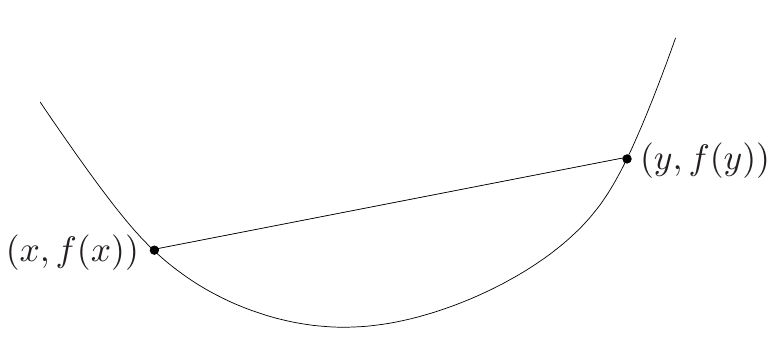
\includegraphics[width=0.7\textwidth]{assets/2 Convex functions/2.1 Concepts and examples/convex function.png}
  \caption{Convex Function}
\end{figure}

A function is strictly convex if strict inequality holds in (5) for all $x \neq y$ and
$\lambda \in (0, 1)$. On the contrary, a function $f$ is concave if $-f$ is convex and
strictly concave if $-f$ is strictly convex.

For an affine function, the inequality (5) holds with equality, meaning that affine
functions are both convex and concave.

There is an important property that a function $f$ is convex if and only if for all
$x \in \textbf{dom } f$ and all $v$, the function $g(t) = f(x + tv)$ is convex in $t$.
This property is useful when checking the convexity of a high-dimensional function.

\subsection{Extended-value extensions}

If $f$ is convex, we define its extended-value extension
\[
\tilde{f}(x) = \begin{cases}
f(x) & x \in \textbf{dom } f \\
\infty & x \notin \textbf{dom } f
\end{cases}
\]

Prof. Ling gives a humorous metaphor here. Imagine $f(x)$ as a pot, it's extended-value
extension is still the pot itself in the pot area, and reaches the sky outside of it, or,
a super pot.

Extended-value extensions are often easier than working with the original function. When
talking about many functions, actually, we talk about its extended-value extension. So
Prof. Boyd said in his book that he will not distinguish between the two, it can be assumed
that all convex functions are implicitly extended.

Here's an example of indicator function of a convex set $C$:
\[
I_c(x) = \begin{cases}
0 & x \in \textbf{dom } C \\
\infty & x \notin \textbf{dom } C
\end{cases}
\]

No doubt, it's convex.

There is one thing to note, the value out of the domain must be $\infty$ or you will get
a non-convex and non-concave function.

In a similar way, we can extend a concave function by defining it to be $-\infty$ outside
its domain.

\subsection{First-order and second-order conditions}

If $f$ is differentiable, then $f$ is convex if and only if $\textbf{dom } f$ is convex and
\[
f(y) \geq f(x) + \nabla f(x)^T (y - x)
\]

\begin{figure}[H]
  \centering
  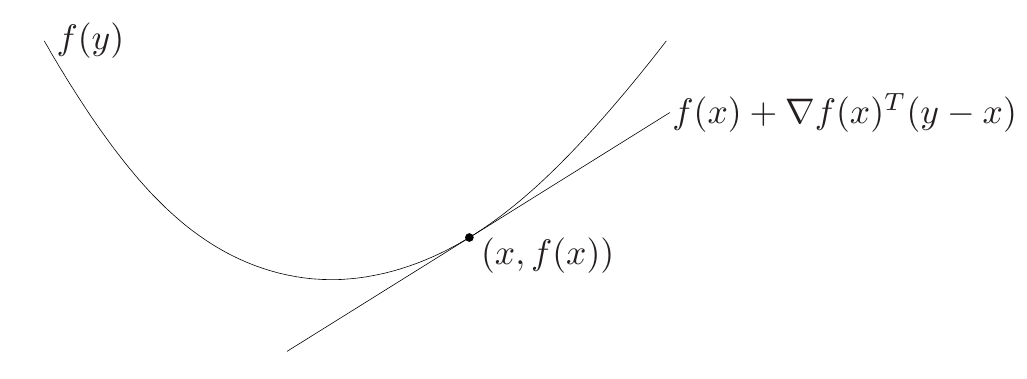
\includegraphics[width=0.7\textwidth]{assets/2 Convex functions/2.1 Concepts and examples/first-order condition.png}
  \caption{First-order Condition}
\end{figure}

The proof of first-order conditions is much complicated, so we won't go into it here.

If $f$ is twice differentiable, then $f$ is convex if and only if $\textbf{dom } f$ is
convex and
\[
\nabla^2 f(x) \succeq 0
\]

$\nabla^2 f(x)$ is called the Hessian matrix.

For a function on $\mathbb{R}$, second-order condition reduces to $f''(x) \geq 0$. In geometry,
this means that the graph of the function has positive curvature on $x$.

Need to note that a strictly convex function don't always meet $\nabla^2 f(x) \succ 0$. For
example, $f(x) = x^4$ is strictly convex, but $f''(0) = 0$.

Consider the quadratic function $f: \mathbb{R}^n \rightarrow \mathbb{R}$ which
$\textbf{dom } f = \mathbb{R}^n$, given by
\[
f(x) = \frac12 x^T P x + q^T x + r,
\]
with $P \in \mathbb{S}^n$, $q \in \mathbb{R}^n$, and $r \in \mathbb{R}$. Since
$\nabla^2 f(x) = P$, $f$ is convex if and only if $P \succeq 0$. And quadratic function
is one of the few strictly convex functions that derives $\nabla^2 f(x) \succ 0$.

It is important that $\textbf{dom } f$ be convex cannot be dropped. If the domain of a
function is not a convex set, it has no possibility to be a convex function. $\frac{1}{x^2}$
is a typical example.

\subsection{Examples}

We have known that linear and affine functions are convex and concave, and the convexity of
quadratic functions. Now we will introduce more functions.

\subsubsection{Exponentials} $e^{ax}$ is convex on $\mathbb{R}$ for any $a \in \mathbb{R}$.

\subsubsection{Powers} $x^a$ is convex on $\mathbb{R}_{++}$ when $a \geq 1$ or $a \leq 0$,
otherwise it's concave.

\subsubsection{Powers of absolute value} $|x|^p$ is convex on $\mathbb{R}$ when $p \geq 1$.

\subsubsection{Logarithm} $\log x$ is concave on $\mathbb{R}_{++}$. Note that $\log x$ here
represents $\ln x$.

\subsubsection{Negative entorpy} $x\log x$ on $\mathbb{R}_{++}$ (define as 0 for $x = 0$)
is convex.

These functions can all be judged for convexity using second-order conditions. We will
talk about a few interesting functions below.

\subsubsection{Norms} Norms are not just $l_p$ norms, they are only part of the norm family.
A norm $P(x)$ has 3 properties:
\begin{itemize}
  \item $P(ax) = |a|P(x)$
  \item $P(x + y) \leq P(x) + P(y)$
  \item $P(x) = 0 \Leftrightarrow x = 0$
\end{itemize}

Norms on $\mathbb{R}^n$ are convex.

\subsubsection{Max function} $f(x) = \max\{x_1, x_2, \ldots, x_n\}$ is convex on $\mathbb{R}^n$.

\subsubsection{log-sum-exp} $f(x) = \log(\sum_{i=1}^{n}e^{x_i})$ is convex on $\mathbb{R}^n$.
This function is a differentiable approximation of the max function:
\[
\max\{x_1, x_2, \ldots, x_n\} \leq f(x) \leq \max\{x_1, x_2, \ldots, x_n\} + \log n
\]

To prove the convexity we need Cauchy-Schwarz inequality, this is a bit complicated so we
omit it here.

\subsubsection{Geometric mean} $f(x) = (\prod_{i = 1}^n x_i)^{\frac{1}{n}}$ is concave on
$\mathbb{R}_{++}$. This proof also uses Cauchy-Schwarz inequality.

\subsubsection{Log-determinant} $f(X) = \log \det X$ is concave on $\mathbb{S}^n_{++}$.

This proof is interesting. Define $X = Z + tV$, where $V \in \mathbb{S}^n$,
$Z \in \mathbb{S}^n_{++}$ and $t \in \mathbb{R}$ then we have:
\begin{align}
f(X) &= \log \det (Z + tV) \\
&= \log \det (Z^{\frac12}(I + tZ^{-\frac12}VZ^{-\frac12})Z^{\frac12}) \\
&= \log \det Z + \sum_{i = 1}^{n} \log (1 + t \lambda_i)
\end{align}
where $\lambda_i$ is the eigenvalues of $Z^{-\frac12}VZ^{-\frac12}$.

It's not easy to understand how (7) becomes (8). Here we will explain deeper.

Since $Z^{-\frac12}VZ^{-\frac12}$ is symmetric, we can perform its spectral decomposition.
Also we know $I = QQ^T$:
\begin{align*}
\det (I + tZ^{-\frac12}VZ^{-\frac12}) &= \det (QQ^T + tQ \Lambda Q^T) \\
&= \det (QQ^T) \det (I + t\Lambda) \\
&= \det (I + t\Lambda) \\
&= \prod_{i = 1}^n 1 + t\lambda_i
\end{align*}

Define $g(t) = f(Z + tV)$, we know
\[
g''(t) = - \sum_{i = 1}^n \frac{\lambda_i^2}{(1 + t\lambda_i)^2} < 0,
\]

So it's concave.

\subsection{Jensen's inequality and extensions}

I knew the convexity of a function when i was in high school, also the Jensen's inequality.
Jensen found a very simple inequality
\[
f(\frac{x + y}{2}) < \frac{f(x) + f(y)}{2}.
\]
Later generations have generalized it into many inequalities, all named after Jensen.

The famous inequalities are
\[
f(\theta x + (1 - \theta) y) < \theta f(x) + (1 - \theta) f(y)
\]
and the generalization
\[
f(\sum_{i = 1}^n \theta_i x_i) < \sum_{i = 1}^n \theta_i f(x_i)
\]
where $f$ is convex, $x_i \in \textbf{dom } f$ and $\theta_i > 0$ with $\sum_{i = 1}^n \theta_i = 1$.

Moreover, we can put these into infinite sums, integrals and so on. Here is the integral
form:
\[
f(\int_S p(x)x dx) < \int_S f(x)p(x) dx
\]
where $p(x) > 0$ on $S \in \textbf{dom } f$ and $\int_S p(x) dx = 1$.

\section{Operations that preserve convexity}
\subsection{Nonnegative weighed sums}

$\alpha f$ is convex if $\alpha > 0 $ and $f$ is convex. $f_1 + f_2$ is convex if $f_1$
and $f_2$ is convex. Now we see that the combination of scaling and addition is a convex
cone, or, a nonnegative weighted sum of convex functions
\[
f = \sum_{i = 1}^n \omega_i x_i,
\]
is convex. Also we can infer that positive weighted sums of convex functions are strictly
convex.

Before we proceed to generalize this definition, we need to talk about the meaning of
jointly convex and separate convex.

$f(x, y)$ is jointly convex when it obeys
\[
f(\theta x_1 + (1 - \theta) x_2, \theta y_1 + (1 - \theta) y_2) \leq \theta f(x_1, y_1) + (1 - \theta) f(x_2, y_2)
\]
where $\theta \in [0, 1]$. And when it's convex in $x$ or $y$ we said that $f(x, y)$ is
separate convex.

If $f(x, y)$ is convex in $x$ and $w(y) > 0$ for each $y \in \mathcal{A}$, then
\[
g(x) = \int_{\mathcal{A}} w(y) f(x, y) dy
\]
is convex.

\subsection{Composition with an affine mapping}

Suppose $f: \mathbb{R}^n \rightarrow \mathbb{R}$, $A \in \mathbb{R}^{n \times m}$ and
$B \in \mathbb{R}^n$. Define $g: \mathbb{R}^m \rightarrow \mathbb{R}$:
\[
g(x) = f(A x + b)
\]
with $\textbf{dom } g = \{x \;|\; A x + B \in \textbf{dom } f\}$. Then the convexity of
$g$ is the same as $f$.

\subsection{Pointwise maximum and supremum}

If $f_1, f2, \ldots, f_n$ are convex, then their pointwise maximum
\[
f(x) = \max\{f_1, f_2, \ldots, f_n\}
\]
with $\textbf{dom } f = \bigcap_{i = 1}^n f_n$ is convex.

Take an example of the sum of $r$ largest components in a set. For $x \in \mathbb{R}^n$
we denote the $i$th largest component by $x_{[i]}$ then the function
\[
f(x) = \sum_{i = 1}^r x_{[i]}
\]
is convex.

Why? This can be rewritten into
\[
f(x) = \max\{\sum_{i = 1}^r x_{[i]} \;|\; 1 \leq x_{[1]} < x_{[2]} < \cdots \leq n\}.
\]
And this is the pointwise maximum of $\binom{n}{r}$ affine functions, so convex.

Like the sum extends to integral when it's infinite, maximum extends to supremum.
This means that the supremum is the least upper bound of the set of values
$\{f(x)\,|\,x\in\mathcal{A}\}$. In other words, a number $\alpha$ is
\[
\alpha=\sup_{x\in\mathcal{A}} f(x)
\]

If $f(x, y)$ is convex in $x$, then
\[
g(x) = \sup_{x\in\mathcal{A}} f(x, y)
\]
is convex. The domain of $g$ is
\[
\textbf{dom } g = \{ x \;|\; (x, y) \in \textbf{dom } f, y \in \mathcal{A}, \sup_{x\in\mathcal{A}} f(x, y) < \infty \}.
\]

Here's an example of maximum eigenvalue of a symmetric matrix
\[
f(X) = \lambda_{\max}(X)
\]
with $\textbf{dom } f = \mathbb{S}^m$ is convex.

Think about the rayleigh quotient
\[
x y = \lambda y \Leftrightarrow \lambda = \frac{y^T x y}{||y||_2^2}.
\]
If we set $||y||_2^2 = 1$, then we can express $f$ as
\[
f(X) = \sup\{y^T X y \;|\; ||y||_2^2 = 1\},
\]
a pointwise supremum of $y^T X y$, a linear function of $X$. The convexity preserves.

\subsection{Composition}

This part we will examine the composition of functions $h: \mathbb{R}^k \rightarrow \mathbb{R}$,
$g: \mathbb{R}^n \rightarrow \mathbb{R}^k$ and $f: h \circ g: \mathbb{R}^n \rightarrow \mathbb{R}$,
defined as
\[
f(x) = h(g(x)), \quad \textbf{dom } f = \{x \in \textbf{dom } g \;|\; g(x) \in \textbf{dom } h\}.
\]

When $k = n = 1$, $h$ and $g$ can be twice differentiable and
$\textbf{dom } g = \textbf{dom } h = \textbf{dom } f = \mathbb{R}$, we can derives that
\[
f''(x) = h''(g(x)){g'(x)}^2 + h'(g(x))g''(x).
\]

Based on the calculations, the following conclusions can be drawn:
\begin{itemize}
  \item $g$ is convex, $h$ is convex, non-decreasing, leads that $f$ is convex.
  \item $g$ is concave, $h$ is convex, non-increasing, leads that $f$ is convex.
\end{itemize}
If it is expected that $f$ is concave, just change the convexity of $h$ and $g$.

Else when $n > 1$, $h$ and $g$ cannot be twice differentiable and
$\textbf{dom } g \neq \mathbb{R}^n$, $\textbf{dom } h \neq \mathbb{R}^k$, we know that:
\begin{itemize}
  \item $f$ is convex if $g$ is convex, $h$ is convex and $\tilde{h}$ is non-decreasing.
  \item $f$ is convex if $g$ is concave, $h$ is convex and $\tilde{h}$ is non-increasing.
\end{itemize}
$\tilde{h}$ here means the extended-value extensions. As the same, changing the convexity of
$h$ and $g$ changes the convexity of $f$.

There are some simple results:
\begin{itemize}
  \item If $g$ is convex, $\exp(g(x))$ is convex.
  \item If $g$ is concave and $g > 0$, $\log(g(x))$ is concave, $1/g(x)$ is convex.
  \item If $g$ is convex and nonnegative, $g(x)^p$ ($p > 1$) is convex.
  \item If $g$ is convex, $-\log(-g(x))$ is convex when $g(x) < 0$.
\end{itemize}

If $k > 1$, we come into vector composition. Suppose
\[
f(x) = h(g_1(x), g_2(x), \ldots, g_k(x))
\]
with $h: \mathbb{R}^k \rightarrow \mathbb{R}$, $g_i: \mathbb{R}^n \rightarrow \mathbb{R}$.

It's more complicated so we omit the process and give out the result here. Thanks that
it's similar to the $n > 1$ situation.

\begin{itemize}
  \item $f$ is convex if $g_i$ is convex, $h$ is convex and $h$ is non-decreasing
  in each argument.
  \item $f$ is convex if $g_i$ is concave, $h$ is convex and $h$ is non-increasing
  in each argument.
\end{itemize}

\subsection{Perspective of a function}
If $f: \mathbb{R}^n \rightarrow \mathbb{R}$, the perspective of $f$ is
$g: \mathbb{R}^n \times \mathbb{R}_{++} \rightarrow \mathbb{R}$ defined by
\[
g(x) = tf(x/t)
\]
with $\textbf{dom } f g\{ (x, t) \;|\; x/t \in \textbf{dom } f, t > 0 \}$. This preserves
convexity.

Think about the square of Euclidean norm
\[
f(x) = x^T x, \quad \textbf{dom } f = \mathbb{R}^n,
\]
its perspective is
\[
g(x, t) = \frac{x^T x}{t}.
\]
which is convex, obviously.

What about the negative logarithm? Consider $f(x) = -\log(x)$ on $\mathbb{R}_{++}$, the
perspective is
\[
g(x, t) = t\log(t) - tlog(x),
\]
and convex on $\mathbb{R}^2_{++}$. This is often called relative entropy of $x$ and $t$.
For $x = 1$, $g$ reduces to the negative entropy.

The relative entropy of 2 vectors $u, v \in \mathbb{R}^n_{++}$ defined as
\[
\sum_{i = 1}^n u_i \log(u_i/v_i)
\]
is convex on $(u, v)$.

There is a closely related function named Kullback-leibler divergence or
\textbf{K-L divergence} given by
\[
D_{kl}(u, v) = \sum_{i = 1}^{n} (u_i \log(u_i/v_i) - u_i + v_i),
\]
which is convex because it's the addition between the relative entropy and an affine
function. Also K-L divergence satisfies
\[
D_{kl}(u, v) \geq 0
\]
and strictly greater than 0 when $u \neq v$.

K-L divergence is a special case of Bregman divergence, and it's widely used for it's
convexity.

\section{The conjugate function}
\subsection{Definition}

Assume $f: \mathbb{R}^n \rightarrow \mathbb{R}$. The function
$f^*: \mathbb{R}^n \rightarrow \mathbb{R}$ defined as
\[
f^*(y) = \sup_{x \in \textbf{dom } f} (y^T x - f(x)),
\]
is called the conjugate of $f$.

There are 2 properties of conjugate function:
\begin{itemize}
  \item If $f$ is differentiable, the corresponding $x$ must satisfy $f'(x) = y$.
  \item The conjugate function is convex.
\end{itemize}

The first one is evident, the second one is because pointwise supremum preserves the convexity of
the affine function.

\begin{figure}[H]
  \centering
  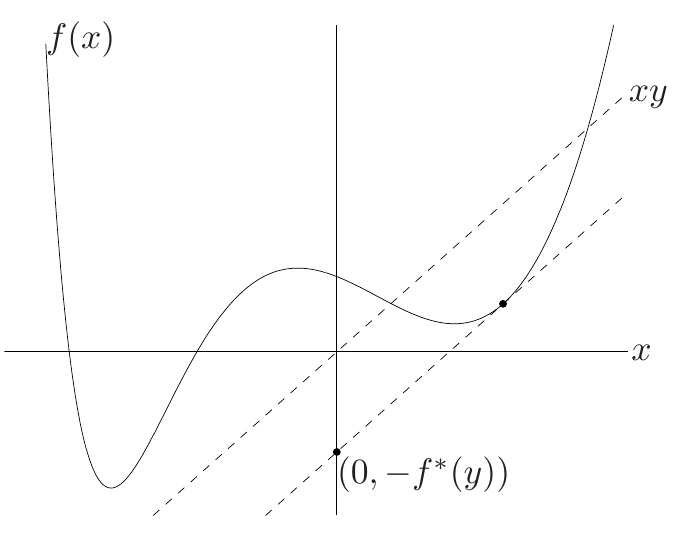
\includegraphics[width=0.6\textwidth]{assets/2 Convex functions/2.3 The conjugate function/conjugate function.png}
  \caption{Conjugate Function}
\end{figure}

\subsection{Examples}

We derive the conjugates of some convex functions on $\mathbb{R}$:
\begin{itemize}
  \item \textbf{Affine function} $f(x) = ax + b$. $\textbf{dom } f^* = \{a\}$ and
  $f^*(a) = -b$.
  \item \textbf{Negative logarithm} $f(x) = -\log(x)$ with $\textbf{dom } f = \mathbb{R}_{++}$.
  $f^*(y) = -\log(-y) - 1$ with $\textbf{dom } f^* = -\mathbb{R}_{++}$.
  \item \textbf{Exponential} $f(x) = e^x$. $f^*(y) = y\log(y) - y$ with
  $\textbf{dom } f^* = \mathbb{R}_+$.
  \item \textbf{Negative entropy} $f(x) = x\log(x)$ with $\textbf{dom } f = \mathbb{R}_+$.
  $f^*(y) = e^{y-1}$.
  \item \textbf{Inverse} $f(x) = 1/x$ on $\mathbb{R}_{++}$. $f^*(y) = -2 \sqrt{-y}$ on
  $-\mathbb{R}_+$.
\end{itemize}

Moreover, consider the strictly convex quadratic funtion $f(x) = \frac12 x^T Q x$ with
$Q \in \mathbb{S}^n_{++}$. First we know
\begin{align*}
  \frac{\partial (y^T x - \frac12 x^T Q x)}{\partial x} &= y - Qx = 0 \\
  &\Rightarrow x = Q^{-1} y.
\end{align*}
Substituting, we get
\[
f^*(y) = \frac12 y^T Q^{-1} y.
\]

There is an interesting question that does the conjugate of a conjugate function equals
itself, or, $f^{**} = f$? The famous example is the imaginary number $a + jb$, but what
about the other?

To be frank I don't like long and complicated proof process, so I will give a wonderful
counterexample. We already know that the conjugate function is convex. So is $f^{**}$.
Assume a concave $f$, these two conflict. Therefore, the answer is no. Actually this
is only correct when $f$ is convex.

\section{Quasiconvex functions}
\subsection{Sublevel sets}

The $\alpha$-sublevel set of a function $f: \mathbb{R}^n \rightarrow \mathbb{R}$ is defined
as
\[
C_{\alpha} = \{ x \in \textbf{dom } f\;|\; f(x) \leq \alpha \}.
\]

Sublevel sets of a convex function is also convex. However, the converse is false. Though
a function has all its sublevel sets convex, it may not be convex. For example, check $-e^x$.

Human beings are creatures in 3D world. However, many mathematical problems lie on a 2D
paper. Hence, these problems are put into 2D coordinate system. We like to talk about
a problem in 2D first, then generalize to higher dimensions. 

Suppose $f: \mathbb{R}^2 \rightarrow \mathbb{R}$, $x \in \mathbb{R}^2$ defined as
\[
f(x) = x^T x.
\]
Certainly we know that its contour lines of this function form concentric circles
centered at the origin, with function values increasing as you move outward from the
origin. Yes, every circle and its inner form a sublevel set. We understand $f(x)$ is
convex, so these sets are convex with no doubt. However, what if we don't know $f(x)$?
With these convex sets, we cannot infer $f(x)$ is convex. This is counterintuitive.

\subsection{Quasiconvex functions}

A function $f: \mathbb{R}^n \rightarrow \mathbb{R}$ is called quasiconvex if its domain
and all sublevel sets
\[
S_{\alpha} = \{ x \in \textbf{dom } f\;|\; f(x) \leq \alpha \}.
\]
are convex. Similarly, a function is called quasiconcave if its domain and all superlevel
sets $\{ x \;|\; f(x) \geq \alpha \}$ are convex. A quasiconvex and quasiconcave function
is called quasilinear.

Quasiconvex functions are similar to convex functions. Many properties hold or have analogs.
For example, quasiconvexity is characterized by the variation of Jensen's inequality:
\[
f(\theta x + (1 - \theta) y) \leq \max\{ f(x), f(y) \}
\]
where $\textbf{dom } f$ is convex and $\theta \in [0, 1]$.

\begin{figure}[H]
  \centering
  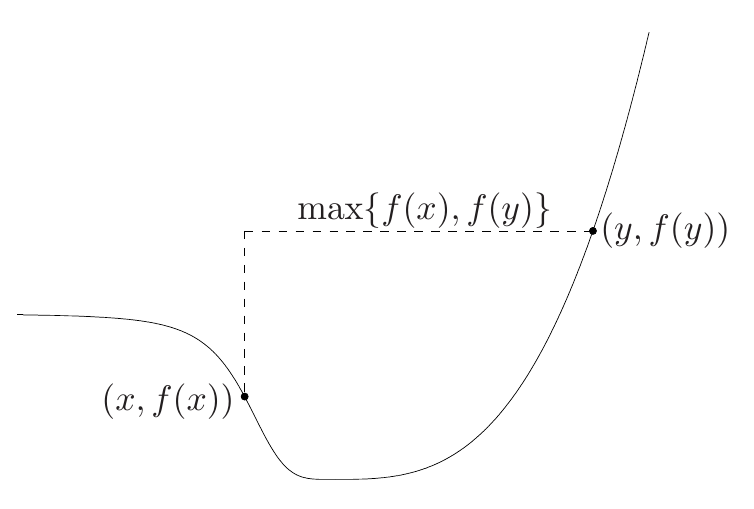
\includegraphics[width=0.6\textwidth]{assets/2 Convex functions/2.4 Quasiconvex functions/quasiconvex function.png}
  \caption{Quasiconvex Function}
\end{figure}

Take an example of the length of a vector or the largest index of a nonzero component
\[
f(x) = \max \{ i \;|\; x_i \neq 0 \}.
\]

This function is quasiconvex. Because that we have
\[
f(x) \leq \alpha \Leftrightarrow x_i = 0 \text{ for } i = \lfloor \alpha \rfloor + 1, \ldots, n.
\]
This function can be seen as a subspace so they are convex, leading to the quasiconvexity.

Another example is the linear fractional function
\[
f(x) = \frac{a^{T}x + b}{c^{T}x + d} \text{ where } \textbf{dom } f = \{x \;|\; c^{T}x + d > 0\}.
\]
Its $\alpha$-sublevel set is
\[
S_{\alpha} = \{x \;|\; c^{T}x + d > 0, \; a^{T}x + b \leq \alpha (c^{T}x + d)\}
\]
It is a convex polyhedron, so quasiconvex. In the same way we know its superlevel set is
also a polyhedron. Therefore, linear fractional function is quasilinear.

Till now, Prof. Ling began to talk about the problem of minimizing $l_0$ norm. I don't
want to write detailed here because my Introduction to Compressed Sensing contains this
part. All you need to know is that the contour lines or the sublevel set of $l_0$ and
$l_1$ norm are the origin and a diamond centered at the origin respectively.

Besides, problems such as
\[
\min ||x||_0 \; s.t. \; x \in C
\]
are hard to solve. People often change the constraints to $||x||_1$ or $x^T x + 1$ or
something else. These two are convex and quasiconvex respectively.

\subsection{First-order and second-order conditions}
Suppose $f: \mathbb{R}^n \rightarrow \mathbb{R}$ is differentiable. The first-order
condition is
\[
f(y) \leq f(x) \Rightarrow \nabla f(x)^T (y - x) \leq 0.
\]
where $\textbf{dom } f$ is convex.

Though convex functions and quasiconvex functions are similar, they still have differenens.
The most important one is that the point satisfies $\nabla f(x) = 0$ may be \textbf{NOT}
the global minimizer of $f(x)$. In other words, this is useless.

Now suppose $f$ is twice differentiable. The second-order condition is
\[
y^T f(x) = 0 \Rightarrow y^T \nabla^2 f(x) y \geq 0.
\]
For a quasiconvex function on $\mathbb{R}$, this reduces to
\[
f'(x) = 0, \; f''(x) \geq 0.
\]
This is said that only those points satisfying $f'(x) = 0$ can use second-order condition.
Hence, without thinking is not a proper choice.

\section{Log-convex and log-concave functions}
A function $f: \mathbb{R}^n \rightarrow \mathbb{R}$ is logarithmically convex or log-convex
if $f(x) > 0$ and $\log(f)$ is convex. Thus $f$ is log-convex if and only if $1/f$ is
log-concave.

Log-convex is stronger than convex, log-concave is weaker than concave. That is to say,
there are 2 properties:
\begin{itemize}
  \item a log-convex function is convex.
  \item a concave function is log-concave.
\end{itemize}

If, like me, you are following Prof. Ling's course while reading the textbook,
you'll notice that the textbook covers much more material beyond this point, but the
course skips it for now. If there's an opportunity, I will add these parts in a later
edition.

\newpage
\chapter{Convex Optimization Problems}
\section{Optimization problems}
\subsection{Basic terminology}
We use
\begin{align}
  \text{minimize } (\min) \; &f_0(x) \nonumber\\
  \text{subject to (s.t.)}\; &f_i(x) \leq 0, \; i = 1, 2, \ldots, m \\
  &h_i(x) = 0, \; i = 1, 2, \ldots, p \nonumber
\end{align}
to describe a simple optimization problem. $x \in \mathbb{R}$ is called optimization
variable. $f_0: \mathbb{R}^n \rightarrow \mathbb{R}$ is called objective function or
cost function (if maximize $f_0$ is called utility function). $f_i(x) \leq 0$ is called
inequality constraints. $h_i(x) = 0$ is called equality constraints. If $m = p = 0$, it
is called unconstrained.

The domain of the optimization problem is defined as
\[
\mathcal{D} = \bigcap_{i = 0}^m \textbf{dom } f_i \cap \bigcap_{i = 0}^p \textbf{dom } h_i.
\]
A point $x \in \mathcal{D}$ is feasible if it satisfies the constraints. The problem is
feasible if there exists at least 1 feasible point. The set of all feasible points is called
feasible set or constraint set.

The optimal value $p^*$ is defined as
\[
p^* = \inf \{f_0(x) \;|\; x \in X_f\}
\]
where $\inf$ represents the infimum and $X_f$ is the feasible set. If the problem is
infeasible $p^* = \infty$. The optimal point (optimal solution) $x^*$ is defined as
$f_0(x^*) = p^*$. And the optimal set is defined as
\[
X_{opt} = \{x \;|\; x \in X_f, \; f_0(x) = p^*\}.
\]
If there exists any optimal point, we say the optinal value is attained or achieved and
the problem is solvable.

A feasible point $x$ with $f_0(x) \leq p^* + \epsilon$ where $\epsilon > 0$ is called
$\epsilon$-suboptimal, the set of all $\epsilon$-suboptimal points is called the $\epsilon$-
optimal set $x_{\epsilon}$.

We say a feasible point $x$ is locally optimal if there is an $R > 0$ such that
\[
f_0(x) = \inf \{ f_0(z) \;|\; z \in X_f, \; ||z - x||_2 \leq R \}.
\]
The set of all locally optimal point is called locally optimal set $x_{loc}$. When the
objective function is convex, $x_{opt} = x_{loc}$.

If $x \in X_f$, $f_i(x) = 0$, then the inequality constraints is active, otherwise
$f_i(x) < 0$, inactive.

Sometimes we don't have an objective function, then the optimization problem becomes
feasibility problem
\begin{align*}
  \text{find } \; &x \\
  \text{s.t. }\; &f_i(x) \leq 0, \; i = 1, 2, \ldots, m \\
  &h_i(x) = 0, \; i = 1, 2, \ldots, p.
\end{align*}

\subsection{Expressing problems in standard form}
We refer (9) as an standard form of optimization problems. We obeys that the right side
of the constraints are 0.

One of the most common problems is the box constraints.
\begin{align*}
  \min \; &f_0(x) \\
  \text{s.t.}\; &l_i \leq x_i \leq u_i,\quad i = 1,2,\ldots,n
\end{align*}

We often express this problem in standard form
\begin{align*}
  \min \; &f_0(x) \\
  \text{s.t.}\; &l_i - x_i \leq 0,\quad i = 1,2,\ldots,n \\
  &x_i - u_i \leq 0,\quad i = 1,2,\ldots,n
\end{align*}

\subsection{Equivalent problems}
Two problems are equivalent if their optimal sets are the same. The constraint functions
can be different, even the form can be totally contrary. The aim of equivalence is to
changing a hard problem to an easier one.

To complete such work, we can often do a function transformation. Here is an example.
Suppose $\psi_0: \mathbb{R} \rightarrow \mathbb{R}$ is monotone increasing,
$\psi_1, \ldots, \psi_m: \mathbb{R} \rightarrow \mathbb{R}$ satisfy $\psi_i(x) \leq 0$
if and only if $x < 0$, $\psi_{m+1}, \ldots, \psi_{m+p}: \mathbb{R} \rightarrow \mathbb{R}$
satisfy $\psi_i(x) = 0$ if and only if $x = 0$.

Then we can say the problem
\begin{align*}
  \min \; &\psi_0(f_0(x)) \\
  \text{s.t.} \; &\psi_i(f_i(x)) \leq 0, \; i = 1, 2, \ldots, m \\
  &\psi_i(h_i(x)) = 0, \; i = m + 1, m + 2, \ldots, m + p
\end{align*}
is equivalent to (9).

If we want to minimize $||A x - b||_2$, it's the same as minimizing $||A x - b||_2^2$.
The first one is not differentiable when $Ax - b = 0$ and the second won't have this
conundrum.

Next we will introduce some simple ways to eliminate constraint functions.

The first is the equality constraints
\[
h_i(x) = 0, \quad i = 1, 2, \ldots, p.
\]
Suppose $\Phi: \mathbb{R}^k \rightarrow \mathbb{R}^n$, there must be some $z \in \mathbb{R}^k$
such that $x = \Phi(z)$. The optimization problem becomes
\begin{align*}
  \min \; &f_0(\Phi(z)) \\
  \text{s.t.} \; &f_i(\Phi(z)) \leq 0, \; i = 1, 2, \ldots, m.
\end{align*}
We should notice 2 things, the relationship of 2 optimal sets is $x^* = \Phi(z^*)$ and
our goal is to make the problem easier. If eliminating constraints let things be worse,
stop it.

\section{Convex optimization problems}
\subsection{The standard form}
The standard form of a convex optimization problem is
\begin{align*}
  \min \; &f_0(x) \\
  \text{s.t.} \; &f_i(x) \leq 0, \; i = 1, 2, \ldots, m \\
  &a_i^T x = b_i, \; i = 1, 2, \ldots, p.
\end{align*}
which $f_0, \ldots, f_m$ are convex. Compare this between (9), we can conclude that
the objective function and the inequality constraint must be convex, and the equality
constraint must be affine.

Besides, it is evident that the feasible set is convex because it is the intersection of
$m$ sublevel sets and $p$ hyperplanes.

Assume a problem
\begin{align*}
  \min \; &f_0(x) = x_1^2 + x_2^2 \\
  \text{s.t.} \; &f_i(x) = \frac{x_1}{1+x_2^2} \leq 0, \; i = 1, 2, \ldots, m \\
  &h_i(x) = {(x_1 + x_2)}^2 = 0, \; i = 1, 2, \ldots, p,
\end{align*}
we can express it in a `convex' way:
\begin{align*}
  \min \; &f_0(x) = x_1^2 + x_2^2 \\
  \text{s.t.} \; &f_i(x) = x_1 \leq 0, \; i = 1, 2, \ldots, m \\
  &h_i(x) = x_1 + x_2 = 0, \; i = 1, 2, \ldots, p,
\end{align*}

\subsection{Slack variables}
Decreasing constraint functions usually makes the problems easier. However, there are
counterexamples such as this form:
\begin{align*}
  \min \; &f_0(x) \\
  \text{s.t.} \; &s_i \geq 0 \; i = 1, 2, \ldots, m \\
  &f_i(x) + s_i = 0, \; i = 1, 2, \ldots, m \\
  &h_i(x) = 0, \; i = 1, 2, \ldots, p,
\end{align*}
where $s_i$ is called the slack variable. It replaces inequality constraints to equality
constraints and nonnegative constraints, which makes certain problems clearly. We will
introduce them later.

\subsection{Some confusing definitions}
If $f_0$ is concave, does we call these concave optimization problems? No. Optimization
problems are divided into 2 kinds, convex and non-convex. Don't make a fool of yourself.

If $f_0$ is quasiconvex, we call these quasiconvex optimization problems, they are
one of the more straightforward part of the non-convex optimization problems.

If $f_0$ is concave and the goal is to maximize it. Now these become concave maximization
problems or convex optimization problems.

Don't get yourself lost.

\section{Local and global optima}
A fundamental property of convex optimization problems is that any local optimal point is
also globally optimal. Suppose $x$ is locally optimal, that is to say, $x$ is feasible and
\[
f_0(x) = \inf \{ f_0(z) \;|\; z \text{ is feasible}, \; ||z - x||_2 \leq R^2 \}
\]
for some $R > 0$.

Assume $x$ is not globally optimal, there must be $y$ satisfies $f_0(y) < f_0(x)$ and
$||y - x||_2 > R$. Consider a $z$ defined as
\[
z = (1 - \theta) x + \theta y, \; \theta = \frac{R}{||y - x||_2}.
\]
Then we have $||z - x||_2 < R$. By the convexity of $f_0$ we have
\[
f_0(z) \leq (1 - \theta) f_0(x) + \theta f_0(y) < f_0(x).
\]
This contradicts. Hence $x$ is globally optimal.

\section{An optimality criterion for differentiable $f_0$}

Suppose the feasible set of a convex optimization problem is $X_f$:
\[
X_f = \{ x \;|\; f_i(x) \leq 0, \; i = 1, 2, \ldots, m \; h_i(x) = 0, \; i = 1, 2, \ldots, p \}.
\]
Then $x^* \in X_f$ is optimal if and only if
\[
\nabla f_0(x^*)^T (y - x^*) \geq 0
\]
where $y$ is an arbitrary value in $X_f$. This is called optimality criterion or optimality
condition.

It can be proved by contradiction. Assume some $y \in X_f$ satisfy
\[
{\nabla f_0(x^*)}^T (y - x^*) < 0.
\]
Consider a line segment $z(t) = ty + (1-t)x, \; t \in [0, 1]$. $z(t)$ is feasible evidently.
Also we have
\[
\left. \frac{d}{dt} f_0(z(t)) \; \right|_{t = 0} = {\nabla f_0(x^*)}^T (y - x^*) < 0.
\]
Hence, there is a small positive $t$ satisfies $f_0(z(t)) < f_0(x)$, which is
impossible.

\subsection{Problems of lacking constraints}
\subsection{Problems with equality constraints only}

Consider a problem with only equality constraints
\begin{align*}
  \min \; &f_0(x) \\
  \text{s.t.} \; &A x = b
\end{align*}

If there is a $x$ satisfies $A x = b$, it's optimal if and only if
\[
\nabla f_0(x)^T (y - x) \geq 0
\]
for any $y$ satisfies $A y = b$. This is equivalent to
\[
\nabla f_0(x)^T v \geq 0
\]
for any $v$ satisfies $A v = 0$, i.e, $v \in \mathcal{N}(A)$.

Here we have 2 cases:
\begin{itemize}
  \item If $v = 0$, then $x = A^{-1} b$ is optimal.
  \item If $v \neq 0$, we know a subspace is closed under scalar multiplication, so
  that $\nabla f_0(x)^T v = 0$ must hold. That is to say,
  $\nabla f_0(x) \in \mathcal{N}(A)^{\perp} = \mathcal{R}(A^T)$ or there is a $\lambda$
  such that $\nabla f_0(x) + A^T \lambda = 0$. This is often called the \textbf{Lagrange
  multiplier condition}.
\end{itemize}

\subsection{Problems with nonnegative constraints only}
Consider a problem with only nonnegative constraints
\begin{align*}
  \min \; &f_0(x) \\
  \text{s.t.} \; &x \succeq 0.
\end{align*}
The optimality criterion is
\[
\nabla f_0(x)^T (y - x) \succeq 0
\]
for any $y \succeq 0$.

Let's talk about it in 2 cases.
\begin{itemize}
  \item If $\nabla f_0(x) \preceq 0$, $\nabla f_0(x)^T y$ reaches $-\infty$ when
  $y \rightarrow \infty$ so the optimality criterion breaks.
  \item If $y = 0$, we have $- \nabla f_0(x)^T x \succeq 0$. But $x \succeq 0$ and
  $\nabla f_0(x) \succeq 0$.
\end{itemize}

Above these, we must have $\nabla f_0(x)^T x = 0$ or
\[
\sum_{i=1}^n (\nabla f_0(x))_i x_i = 0.
\]
Because that $x_i \geq 0$ and $(\nabla f_0(x))_i \geq 0$, we have
\[
(\nabla f_0(x))_i x_i = 0, \; i = 1, 2, \ldots, n.
\]
This is called \textbf{complementarity}.

\section{Linear programs}
\subsection{Concept}

A general linear program (LP) is
\begin{align*}
\min \; &c^T x + d\\
\text{s.t.} \; &Gx \preceq h\\
&Ax = b
\end{align*}
where $G \in \mathbb{R}^{m \times n}, A \in \mathbb{R}^{p \times n}$.

It's common to omit the constant term $d$ because it doesn't change the optimal set.
The geometric interpretation of an LP is shown in the figure below. The feasible set is
a polyhedron $\mathcal{P}$. The dash lines are the contour lines of the objective function.

\begin{figure}[H]
  \centering
  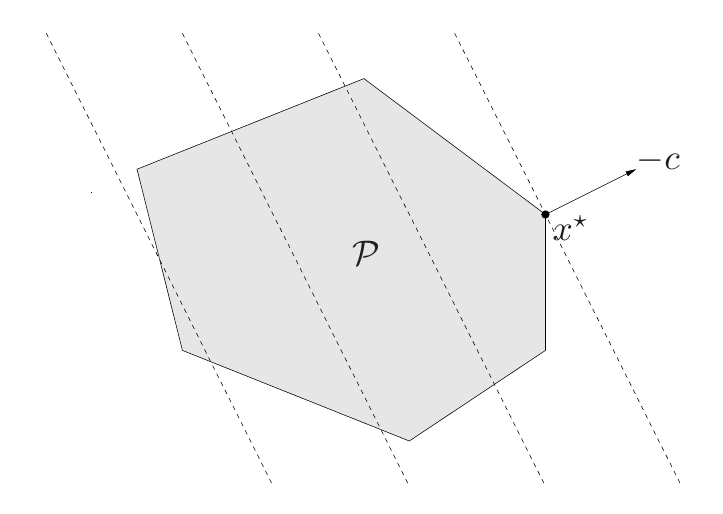
\includegraphics[width=0.6\textwidth]{assets/3 Convex optimization problems/3.5 Linear programs/LP.png}
  \caption{Linear Program}
\end{figure}

\subsection{Converting LPs to standard form}

The first step is to add slack variables $s_i$ which will result in
\begin{align*}
\min \; &c^T x + d\\
\text{s.t.} \; &Gx + s = h\\
&Ax = b\\
&s \succeq 0
\end{align*}

The second step is to divide $x$ into 2 negative parts $x^+$ and $x^-$ where $x = x^+ - x^-$
and $x^+, x^- \succeq 0$. Then we have
\begin{align*}
\min \; &c^T x^+ - c^T x^- + d\\
\text{s.t.} \; &Gx^+ - Gx^- + s = h\\
&Ax^+ - Ax^- = b\\
&x^+, x^- \succeq 0, s \succeq 0
\end{align*}

This is the standard form of an LP. However, most of the time we use the simplest form
\begin{align*}
\min \; &c^T x\\
\text{s.t.} \; &Ax = b\\
&x \succeq 0
\end{align*}
which is called the \textbf{canonical form} of an LP.

\subsection{Diet problem}

LPs arise in many applications. Here we introduce a famous diet problem.

A healthy diet contains $m$ nutrients and not smaller than $b_i$ of the $i$-th nutrient.
There are $n$ food, and the $j$-th food contains $a_{ij}$ of the $i$-th nutrient.
The cost of the $j$-th food is $c_j$. The problem is to find the cheapest diet.
The problem can be formulated as
\begin{align*}
\min \; &c^T x\\
\text{s.t.} \; &Ax \succeq b\\
&x \succeq 0.
\end{align*}

However, some of the food must be integer, which makes the problem nonconvex. So we are
thinking about the problem with only continuous variables or a much easier way.

\subsection{Linear fractional programming}

Linear fractional programming is a special case of linear programming. The problem is
\begin{align*}
\min \; &f_0(x) = \frac{c^T x + d}{e^T x + f}\\
\text{s.t.} \; &Gx \preceq h\\
&Ax = b
\end{align*}
where $e^T x + f > 0$ for any feasible $x$. $f_0(x)$ is quasilinear.

If the feasible set is nonempty, we can rewrite the problem as
\begin{align*}
\min \; &c^T x + dz\\
\text{s.t.} \; &Gy - hz \preceq 0\\
&Ay - bz = 0\\
&e^T y + fz = 1\\
&z > 0,
\end{align*}
where we define
\[
y = \frac{x}{e^T x + f}, \quad z = \frac{1}{e^T x + f}.
\]
It's no doubt that we transfer a linear fractional programming to an LP. The prove of
the equivalence is boring, so I won't write it here.

\subsection{Quadratic programming}
Quadratic programming (QP) is a special case of convex optimization problems. The problem is
\begin{align*}
\min \; &f_0(x) = \frac12 x^T P x + q^T x + r\\
\text{s.t.} \; &Gx \preceq h\\
&Ax = b,
\end{align*}
where $P \in \mathbb{S}^n_+$.

\begin{figure}[H]
  \centering
  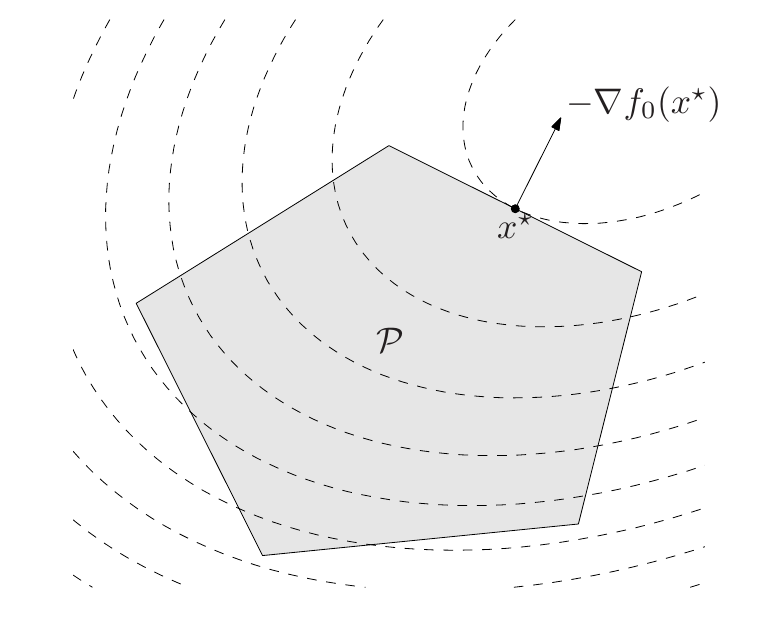
\includegraphics[width=0.6\textwidth]{assets/3 Convex optimization problems/3.5 Linear programs/QP.png}
  \caption{Quadratic Program}
\end{figure}

If we change the constraints to quadratic constraints, we have quadratically constrained
quadratic programming (QCQP):
\begin{align*}
\min \; &f_0(x) = \frac12 x^T P x + q^T x + r\\
\text{s.t.} \; &f_i(x) = \frac12 x^T P_i x + q_i^T x + r_i \leq 0, \; i = 1, 2, \ldots, m\\
&Ax = b,
\end{align*}
where $P, P_1, \ldots, P_m \in \mathbb{S}^n_+$.

QPs include LPs as a special case by setting $P = 0$. QCQPs include QPs as a special case
by setting $P_i = 0$.

Here we give an important example, the least squares problem
\[
\min \; f_0(x) = ||A x - b||_2^2 = x^T A^T A x - 2 b^T A x + b^T b.
\]
This is an unconstrained QP. We know the optimal point is $x^* = A^{\dagger} b$
where $A^{\dagger}$ is the pseudo-inverse of $A$.

Sometimes we have a sparse $x$, then we can add a regularization term$\lambda ||x||_1$
to the objective function. This is called $l_1$ regularization or \textbf{LASSO}.
The problem becomes
\[
\hat{x} = \argmin_{x} ||Ax - b||_2^2 + \lambda ||x||_1.
\]

Moreover, we can also add a $l_2$ regularization term $\lambda ||x||_2^2$, which is
called \textbf{Ridge regression}. The problem becomes
\[
\hat{x} = \argmin_{x} ||Ax - b||_2^2 + \lambda ||x||_2^2.
\]
Ridge regression is a QCQP actually because we can rewrite it as
\begin{align*}
\min \; &||Ax - b||_2^2\\
\text{s.t.} \; &||x||_2^2 \leq t
\end{align*}
where $t$ is a positive constant. The prove will be obvious after we talk about the duality.

\subsection{Portfolio optimization}

We have $B$ budgets and $n$ assets. Every asset was invested $x_i$ dollars, and the return
of the $i$-th asset is $p_i$. $p$ is a random variable, and we know its mean $\bar{p}$ and
covariance matrix $\Sigma$. Therefore the return $r$ is also a random variable with mean
$\bar{p}^T x$ and variance $x^T \Sigma x$. We want to minimize the risk, which is the
variance of the return, while guaranteeing the return is not smaller than $r_{min}$.
The classical portfolio optimization problem is given by Markowitz as
\begin{align*}
\min \; &x^T \Sigma x\\
\text{s.t.} \; &\bar{p}^T x \geq r_{min}\\
&1^T x = B\\
&x \succeq 0.
\end{align*}

\subsection{Semidefinite programming}
Standard semidefinite programs (SDP) has such a form
\begin{align*}
\min \; &\text{tr}(C X)\\
\text{s.t.} \; &\text{tr}(A_i X) = b_i, \; i = 1, 2, \ldots, p\\
&X \succeq 0,
\end{align*}
where $C, A_1, \ldots, A_p \in \mathbb{S}^n$, $X \in \mathbb{S}^n$ and $\text{tr}(\cdot)$
is the trace of a matrix.

One of the special cases is the diagonal semidefinite program, where $C, A_1, \ldots, A_p$
are all diagonal. This can be rewritten as
\begin{align*}
\min \; &(diag(C))^T diag(X)\\
\text{s.t.} \; &(diag(A_i))^T diag(X) = b_i, \; i = 1, 2, \ldots, p\\
&diag(X) \succeq 0,
\end{align*}
where $diag(\cdot)$ is the operator that extracts the diagonal of a matrix.

An inequality form of SDP is
\begin{align*}
\min \; &c^T x\\
\text{s.t.} \; &\sum_{i=1}^n x_i A_i \preceq B,
\end{align*}
where $A_1, \ldots, A_n, B \in \mathbb{S}^k$ and $x, c \in \mathbb{R}^n$.

Let $A(x) = A_0 +\sum_{i=1}^n x_i A_i$ where $A_i \in \mathbb{R}^{p \times q}$, we consider
an unconstrained problem
\[
\min \; ||A(x)||_2.
\]
In linear algebra we know $||A(x)||_2$ is the largest singular value of $A(x)$, and also
we have $||A(x)||_2 < \sqrt{s}$ for some $s > 0$ if and only if $A(x)^T A(x) \prec s I$.
Hence, we can rewrite the problem as
\begin{align*}
\min \; &s\\
\text{s.t.} \; &A(x)^T A(x) \prec s I\\
&s > 0.
\end{align*}

To represent $A(x)^T A(x) \prec s I$ in a SDP way, we should notice that it is equivalent to
\[
\begin{bmatrix}
s I & A(x)\\
A(x)^T & s I
\end{bmatrix} \succeq 0
\]
This is exactly an LMI, or a SDP constraint.

\section{Multicriterion problems}
\subsection{Pareto optimal points and values}

A feasible point $x$ is Pareto optimal if $f_0(x)$ is a minimal element of the set of
achievable values $\mathcal{O}$. That is to say, there is no $y$ such that
$f_0(y) \preceq f_0(x)$ and $f_0(y) \neq f_0(x)$. Also we can define it in a mathematical
way. $x$ is Pareto optimal if and only if
\[
(f_0(x) - K) \cap \mathcal{O} = \{f_0(x)\}
\]
where $K$ is the positive cone. $f_0(x) - K$ represents the set of all values that are
better than $f_0(x)$.

Pareto optimal means that we cannot improve one criterion without worsening another.
The set of all Pareto optimal points is called the Pareto optimal set. The set of all
Pareto optimal values is called the Pareto front.

A optimazation problem can have multiple Pareto optimal points, they form the Pareto front.
The Pareto front must be part of the boundary of the achievable set $\mathcal{O}$.

\subsection{An example}

Let us consider the ridge regression problem again. We have a problem at first, which is
\[
\min \; ||Ax - b||_2^2.
\]
On the one hand, we want to minimize the error $||Ax - b||_2^2$. On the other hand,
we want to minimize the energy $||x||_2^2$, it can be seen as:
\[
\min \; ||Ax - b||_2^2 + \lambda ||x||_2^2.
\]
We can also see it as a multicriterion problem.

\begin{figure}[H]
  \centering
  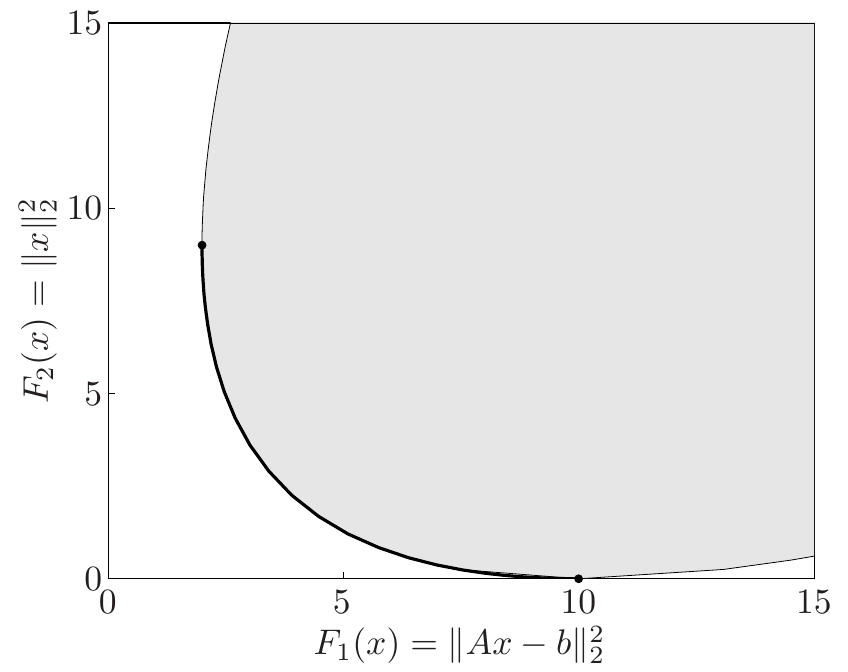
\includegraphics[width=0.6\textwidth]{assets/3 Convex optimization problems/3.6 Multicriterion problem/Ridge regression multicriterion problem.png}
  \caption{Ridge regression as a multicriterion problem}
\end{figure}
The Pareto front is the curve in the figure above. The points on the curve is Pareto optimal.

Notice that most of the multicriterion problems are hard to solve, the ridge regression is
a special case. This part does not intend to introduce the concept of multicriterion problems,
but to give a background for the next chapter, which is about duality.

\newpage
\chapter{Duality}
\section{The Lagrange dual function}
\subsection{The Lagrangian}

Consider an optimization problem in standard form:
\begin{align*}
\min \; &f_0(x)\\
\text{s.t.} \; &f_i(x) \leq 0, \; i = 1, 2, \ldots, m\\
&h_i(x) = 0, \; i = 1, 2, \ldots, p.
\end{align*}
We assume its domain $\mathcal{D} = \bigcap_{i = 0}^m \textbf{dom } f_i \cap \bigcap_{i = 0}^p \textbf{dom } h_i$
is nonempty and there is a optimal value $p^*$.

Define the Lagrangian $L$ as
\[
L(x, \lambda, \nu) = f_0(x) + \sum_{i=1}^m \lambda_i f_i(x) + \sum_{i=1}^p \nu_i h_i(x)
\]
where $\lambda \in \mathbb{R}^m$ and $\nu \in \mathbb{R}^p$ are called the Lagrange
multiplier vectors or dual variables.

\subsection{The Lagrange dual function}

We define the Lagrange dual function (or just dual function) $g$ as
\[
g(\lambda, \nu) = \inf_{x \in \mathcal{D}} L(x, \lambda, \nu).
\]

Lagrange dual function has 2 important properties:
\begin{itemize}
  \item $g$ is always concave.
  \item For any $\lambda \succeq 0$ and $\nu$, we have $g(\lambda, \nu) \leq p^*$.
\end{itemize}

Here is a proof of the second property. Assume $\lambda \succeq 0$ and $\nu$ are arbitrary.
For a optimal point $x^*$, we have
\[
L(x^*, \lambda, \nu) = f_0(x^*) + \sum_{i=1}^m \lambda_i f_i(x^*) + \sum_{i=1}^p \nu_i h_i(x^*).
\]
Because $x^*$ is feasible, we have $f_i(x^*) \leq 0$ and $h_i(x^*) = 0$. Hence,
\[
L(x^*, \lambda, \nu) \leq f_0(x^*) = p^*.
\]
So we know $g(\lambda, \nu) \leq L(x^*, \lambda, \nu) \leq p^*$.

\subsection{Examples}
Consider an LP
\begin{align*}
\min \; &c^T x\\
\text{s.t.} \; &Ax = b\\
&x \succeq 0.
\end{align*}
Notice that $f_i(x) = -x_i$. The Lagrangian is
\[
L(x, \lambda, \nu) = (c - \lambda + A^T \nu)^T x - \nu^T b.
\]
Then the dual function is
\[
g(\lambda, \nu) = \inf_{x} L(x, \lambda, \nu) =
\begin{cases}
- \nu^T b, & c - \lambda + A^T \nu = 0\\
- \infty, & \text{otherwise}.
\end{cases}
\]

Consider a nonconvex 2-way partitioning problem
\begin{align*}
\min \; &x^T W x\\
\text{s.t.} \; &x_i^2 = 1, \; i = 1, 2, \ldots, n.
\end{align*}
The Lagrangian is
\[
L(x, \nu) =  x^T (W + diag(N)) x - 1^T \nu,
\]
where $N$ is a diagonal matrix with $\nu$ on the diagonal. Then the dual function is
\[
g(\nu) = \inf_{x} L(x, \nu) =
\begin{cases}
- 1^T \nu, & W + diag(N) \succeq 0\\
- \infty, & \text{otherwise}.
\end{cases}
\]

\section{The Lagrange dual problem}

We have known that $g(\lambda, \nu) \leq p^*$ for any $\lambda \succeq 0$ and $\nu$.
So we can try to find the best lower bound of $p^*$ by solving the following problem
\begin{align*}
\max \; &g(\lambda, \nu)\\
\text{s.t.} \; &\lambda \succeq 0.
\end{align*}
This is called the Lagrange dual problem. The optimal value of the dual problem is called
the dual optimal value, denoted by $d^*$. We have $d^* \leq p^*$. Also, $\lambda^*, \nu^*$
are called the optimal Lagrange multipliers. Remember that the dual problem is always a
convex optimization problem.

Let's take the former LP as an example again. The dual problem is
\begin{align*}
\max \; &- \nu^T b\\
\text{s.t.} \; &\nu \succeq 0\\
&c - \lambda + A^T \nu = 0.
\end{align*}
Also we can rewrite it as
\begin{align*}
\min \; & \nu^T b\\
\text{s.t.} \; &A^T \nu + c\succeq 0.
\end{align*}
However, the dual optimal value changed because the objective function changed. The optimal
Lagrange multipliers stay the same.

\section{Strong duality and Slater's condition}
\subsection{Definition}
Before we start this part, some important definitions are given.
\begin{itemize}
  \item the inequality $d^* \leq p^*$ is called the weak duality.
  \item if $d^* = p^*$, we call it strong duality.
  \item the duality gap is given by $p^* - d^*$.
\end{itemize}

Moreover, the relative interior of a set $D$ is the interior of $D$ relative to its affine hull,
denoted by $\textbf{relint } D$ and we have
\[
\textbf{relint } D = \{ x \in D \;|\; B(x,r) \cap \textbf{aff } D \in D \; \exists \; r > 0 \}.
\]

There is also a simpler definition of the relative interior. It's the set of all points in
$D$ that are not on the boundary of $D$.

\subsection{Slater's condition}

Slater's condition is a sufficient but not necessary condition for strong duality.It states
that if there is a point
\[
x \in \textbf{relint } \mathcal{D}
\]
satisfies $f_i(x) < 0$ for $i = 1, 2, \ldots, m$ and $h_i(x) = 0$ for $i = 1, 2, \ldots, p$,
then strong duality holds. Such a point is called strictly feasible.

Slater's condition can be refined when some $f_i$ are affine. If the first $k$'s are affine,
then we only need to find a point $x$ such that $f_i(x) < 0$ for $i = k + 1, k + 2, \ldots, m$.
That means we can ignore the affine constraints. Moreover, if constraints are all affine,
the only thing we need to do is to find a feasible point. Obviously, a feasible LP always
satisfies this weaker Slater's condition.

Let's consider QCQP
\begin{align*}
\min \quad &\frac12 x^T P_0 x + {q_0}^T x + r_0\\
\text{s.t.} \quad &x^T P_i x + {q_i}^T x + r_i \leq 0, \; i = 1, 2, \ldots, m,
\end{align*}
with $P_0, P_1, \ldots, P_m \in \mathbb{S}^n_+$ and $P_0 \in \mathbb{S}^n_{++}$.

Slater's condition is satisfied if there is a point $x$ such that
\[
x^T P_i x + {q_i}^T x + r_i < 0, \; i = 1, 2, \ldots, m.
\]
However, if $q_i = r_i = 0$, we cannot find such $x$ because $x^T P_i x \geq 0$ for any $x$.
In this case, Slater's condition is broken. But we can't judge whether strong duality holds
or not. Actually, strong duality still holds in this case. When Slater's condition is broken,
most of the time we have to check the strong duality by hand.

\section{Equivalent problems with different dual problems}
Consider an unconstrained problem
\[
min f_0(Ax + b).
\]
The dual function is just $p^*$, the dual problem is trivial and strong duality holds. However, if we
reformulate the problem as
\begin{align*}
\min \; &f_0(y)\\
\text{s.t.} \; &Ax + b = y,
\end{align*}
the dual function is
\[
g(\nu) = \inf_{x, y} \{f_0(y) + \nu^T (Ax + b - y)\} = \inf_y \{f_0(y) - \nu^T y\} + \inf_x \{\nu^T A x\} + \nu^T b.
\]
Notice that
\begin{align*}
\inf_x \{\nu^T A x\} &= \begin{cases}
0, & A^T \nu = 0\\
- \infty, & \text{otherwise}.
\end{cases}
\end{align*}
So the dual function is
\[
g(\nu) = b^T \nu + \inf_y \{f_0(y) - \nu^T y\} = b^T \nu - f_0^*(\nu), A^T \nu = 0,
\]
where $f_0^*$ is the convex conjugate of $f_0$.
The dual problem is
\begin{align*}
\max \; &b^T \nu - f_0^*(\nu)\\
\text{s.t.} \; &A^T \nu = 0.
\end{align*}

More examples will be given below. Consider a problem
\[
\min \; ||Ax - b||.
\]
It is just an unconstrained problem, so the dual problem is useless. However, if we reformulate it as
\begin{align*}
\min \; &||y||\\
\text{s.t.} \; &Ax - b = y,
\end{align*}
we can get a new dual problem
\begin{align*}
\max \; &b^T \nu\\
\text{s.t.} \; &||\nu||_* \leq 1\\
& A^T \nu = 0,
\end{align*}
where $||\cdot||_*$ is the dual norm of $||\cdot||$, defined as
\[
||y||_* = \sup_{x} \{y^T x \;|\; ||x|| \leq 1\}.
\]

If we reformulate the problem as
\begin{align*}
\min \; &\frac12 ||y||^2\\
\text{s.t.} \; &Ax - b = y,
\end{align*}
They have the same optimal point but different optimal value. The dual problem is
\begin{align*}
\max \; &b^T \nu - \frac12 ||\nu||^2\\
\text{s.t.} \; &A^T \nu = 0.
\end{align*}
This is also different from the former dual problem.

The last one problem is with a implicit constraint
\begin{align*}
\min \; &c^T x\\
\text{s.t.} \; &Ax = b\\
&l \preceq x \preceq u,
\end{align*}
where $A \in \mathbb{R}^{p \times n}$ and $l \preceq u$. The constraints $l \preceq x \preceq u$ is
sometimes called box constraints or variable bounds.

To shorten the derivation, we only give the dual problem here. The dual problem is
\begin{align*}
\max \; &-b^T \nu - \lambda_1^T u + \lambda_2^T l\\
\text{s.t.} \; &A^T \nu + \lambda_1 - \lambda_2 + c = 0\\
&\lambda_1 \succeq 0, \; \lambda_2 \succeq 0.
\end{align*}

Instead, the reformulation of the problem is
\begin{align*}
\min \; &f_0(x)\\
\text{s.t.} \; &Ax = b,
\end{align*}
where we define
\[
f_0(x) = \begin{cases}
c^T x, & l \preceq x \preceq u\\
+ \infty, & \text{otherwise}.
\end{cases}
\]
The dual problem is
\[
\max \; -b^T \nu - u^T (A^T \nu + c)^- + l^T (A^T \nu + c)^+,
\]
where $(\cdot)^+ = \max\{0, \cdot\}$ and $(\cdot)^- = \max\{0, -\cdot\}$. These two dual problems look
different but they are actually the same, though.

\section{Interpretations}
\subsection{Geometric interpretation}
Define a set $G$ as
\[
G = \{ (f_1(x), \ldots, f_m(x), h_1(x), \ldots, h_p(x), f_0(x)) \;|\; x \in \mathcal{D} \}.
\]
And we know that
\[
p^* =  \inf \{ t \;|\; (u, v, t) \in G, u \preceq 0, v = 0\},
\]


The Lagrangian can be written as
\[
L(x, \lambda, \nu) = (\lambda, \nu, 1)^T (u, v, t),
\]
Then the dual function is
\[
g(\lambda, \nu) = \inf\{(\lambda, \nu, 1)^T (u, v, t) \;|\; (u, v, t) \in G\}.
\]

Suppose $\lambda \succeq 0$. Obviously, $t \geq (\lambda, \nu, 1)^T (u, v, t)$ with
$u \preceq 0$ and $v = 0$. Hence,
\begin{align*}
p^* &= \inf \{ t \;|\; (u, v, t) \in G, u \preceq 0, v = 0\} \\
&\geq \inf \{ (\lambda, \nu, 1)^T (u, v, t) \;|\; (u, v, t) \in G, u \preceq 0, v = 0\} \\
&\geq \inf \{ (\lambda, \nu, 1)^T (u, v, t) \;|\; (u, v, t) \in G\} \\
&= g(\lambda, \nu).
\end{align*}
Above these, we prove the weak duality again.

\begin{figure}[H]
  \centering
  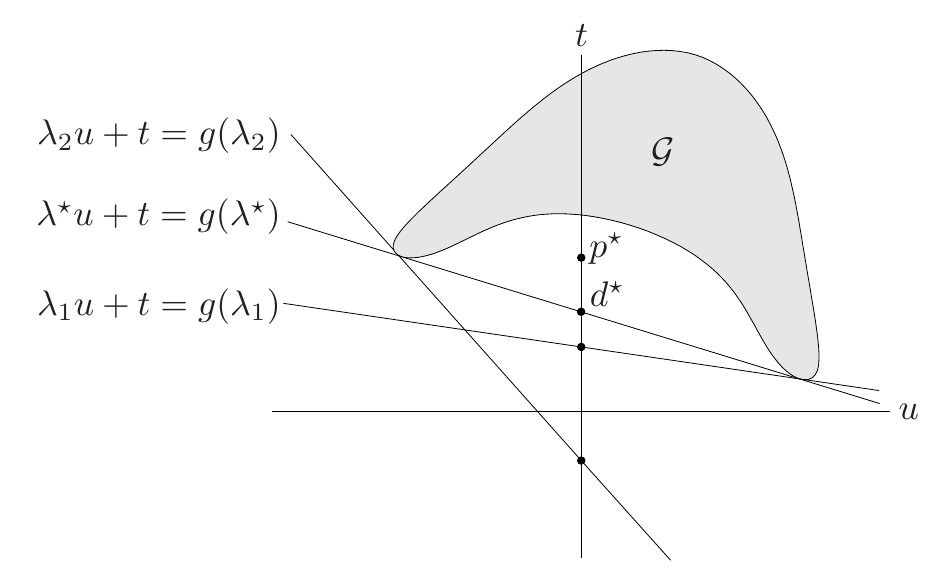
\includegraphics[width=0.7\textwidth]{assets/4 Duality/4.4 Interpretations/Geometric interpretation.png}
  \caption{Geometric interpretation of duality}
\end{figure}

Here's the geometric interpretation. $v$ is omitted for simplicity. $g(\lambda)$ is the
supporting hyperplane of $\mathcal{G}$. The dual problem is to find $g(\lambda^*)$. Its intersection
with the $t$-axis is $d^*$. The primal problem is to find the lowest point $p^*$ of $G$ that
satisfies $u \preceq 0$. We can see that $d^* \leq p^*$.

\subsection{Saddle-point interpretation}
Note that
\begin{align*}
\sup_{\lambda \succeq 0} L(x, \lambda) &= \sup_{\lambda \succeq 0} \{ f_0(x) + \sum_{i=1}^m \lambda_i f_i(x) \} \\
&= \begin{cases}
f_0(x), & f_i(x) \leq 0, \; i = 1, 2, \ldots, m\\
+ \infty, & \text{otherwise}.
\end{cases}
\end{align*}
This means that the primal problem is equivalent to
\[
p^* = \inf_{x} \sup_{\lambda \succeq 0} L(x, \lambda).
\]
At the same time, we have
\[
d^* = \sup_{\lambda \succeq 0} \inf_{x} L(x, \lambda).
\]
Thus, weak duality can be rewritten as
\[
\sup_{\lambda \succeq 0} \inf_{x} L(x, \lambda) \leq \inf_{x} \sup_{\lambda \succeq 0} L(x, \lambda).
\]

Actually, this inequality holds for any function $f(x, y)$, not necessarily the Lagrangian.
And the inequality is called the max-min inequality. When the equality holds, we say that
$f, x, y$ satisfy the saddle-point property.

We call $(x, y)$ a saddle point of $f$ if
\[
f(\tilde{x}, y) \leq f(x, y) \leq f(x, \tilde{y}).
\]
In other words, we have
\[
f(\tilde{x}, \tilde{y}) = \inf_{x} f(x, \tilde{y}) = \sup_{y} f(\tilde{x}, y).
\]
This means that the saddle point is the optimal point of both the primal and dual problems.
Hence, if there is a saddle point of the Lagrangian, strong duality holds.

\subsection{Economic interpretation}
Suppose $f_0(x)$ is the cost of producing $x$ and $f_i(x)$ is the amount of resource $i$
limiting the production. Then we can write the problem as
\begin{align*}
\min \; &f_0(x)\\
\text{s.t.} \; &f_i(x) \leq 0, \; i = 1, 2, \ldots, m.
\end{align*}
The optimal profit is $-p^*$.

Now imagine a different case, the factory can violate the resource but has to pay $\lambda_i$
for each resource $i$. At the same time, it can sell the resource with price $\lambda_i$ if
it has extra resource. The cost now is
\[
L(x, \lambda) = f_0(x) + \sum_{i=1}^m \lambda_i f_i(x).
\]
The factory wants to minimize the cost by choosing $x$ and $\lambda$. The optimal cost is
\[
g(\lambda) = \inf_{x} L(x, \lambda).
\]
Then we can describe $d^* = \sup_{\lambda \succeq 0} g(\lambda)$ as the optimal cost when
$\lambda$ is chosen by external market to make the factory's cost as high as possible.
The weak duality tells us that the optimal cost of the factory in the second case is not
higher than the optimal cost in the first case, which means that the factory cannot make
more profit by violating the resource constraints.

\section{KKT optimality conditions}
\subsection{Complementary slackness}
Assume a simple problem
\begin{align*}
\min \; &f_0(x)\\
\text{s.t.} \; &f_i(x) \leq 0, \; i = 1, 2, \ldots, m.
&h_i(x) = 0, \; i = 1, 2, \ldots, p
\end{align*}
and strong duality holds. We know $x^*, \lambda^*, \nu^*$ must satisfy
\begin{align*}
f_i(x^*) &\leq 0, \; i = 1, 2, \ldots, m\\
h_i(x^*) &= 0, \; i = 1, 2, \ldots, p\\
\lambda^* &\succeq 0.
\end{align*}
Also we have
\begin{align*}
f_0(x^*) &= g(\lambda^*, \nu^*)\\
&= \inf_x \{f_0(x) + \sum_{i=1}^m \lambda_i^* f_i(x) + \sum_{i=1}^p \nu_i^* h_i(x)\}\\
&\leq f_0(x^*) + \sum_{i=1}^m \lambda_i^* f_i(x^*) + \sum_{i=1}^p \nu_i^* h_i(x^*)\\
&= f_0(x^*) + \sum_{i=1}^m \lambda_i^* f_i(x^*)\\
&\leq f_0(x^*).
\end{align*}
This is interesting. From the above inequalities, we have
\[
\sum_{i=1}^m \lambda_i^* f_i(x^*) = 0.
\]
Because $\lambda_i^* \geq 0$ and $f_i(x^*) \leq 0$, we have $\lambda_i^* f_i(x^*) = 0$
for all $i$. This is called the complementary slackness.

\subsection{KKT optimality conditions}
Now we assume that all functions are differentiable. Since $x^*$ minimizes
$L(x, \lambda^*, \nu^*)$, we have $\nabla_x L(x^*, \lambda^*, \nu^*) = 0$ or
\[
\nabla f_0(x^*) + \sum_{i=1}^m \lambda_i^* \nabla f_i(x^*) + \sum_{i=1}^p \nu_i^* \nabla h_i(x^*) = 0.
\]
This is often called the stationarity condition.

Thus all conditions are given by
\begin{align*}
f_i(x^*) &\leq 0, \; i = 1, 2, \ldots, m\\
h_i(x^*) &= 0, \; i = 1, 2, \ldots, p\\
\lambda^* &\succeq 0\\
\lambda_i^* f_i(x^*) &= 0, \; i = 1, 2, \ldots, m\\
\nabla f_0(x^*) + \sum_{i=1}^m \lambda_i^* \nabla f_i(x^*) + \sum_{i=1}^p \nu_i^* \nabla h_i(x^*) &= 0,
\end{align*}
which is called the Karush-Kuhn-Tucker (KKT) optimality conditions. Moreover, KKT conditions
are only necessary but not sufficient for nonconvex problems. It's sufficient and necessary
only for convex problems with zero duality gap and differentiable functions.

This is easy to understand through the process below. We have
\begin{align*}
g(\lambda^*, \nu^*) &= L(x^*, \lambda^*, \nu^*)\\
&= f_0(x^*) + \sum_{i=1}^m \lambda_i^* f_i(x^*) + \sum_{i=1}^p \nu_i^* h_i(x^*)\\
&= f_0(x^*).
\end{align*}
And from this we can see that $x^*$ is the saddle point of $L(x, \lambda^*, \nu^*)$. We have
talked about the saddle-point interpretation of duality, so we know that $x^*$ is the
optimal point of the primal problem.

\subsection{Examples}
Consider a QP problem
\begin{align*}
\min \; &\frac12 x^T P x + q^T x + r\\
\text{s.t.} \; &Ax = b
\end{align*}
where $P \in \mathbb{S}^n_+$. The Lagrangian is
\[
L(x, \nu) = \frac12 x^T P x + q^T x + r + \nu^T (Ax - b).
\]
Then the KKT condition is
\[
Ax^* = b, \; P x^* + q + A^T \nu^* = 0.
\]
The first condition is the primal feasibility, and the second condition is the stationarity.

Next is a water-filling problem
\begin{align*}
\min \; &-\sum_{i=1}^n \log(a_i + x_i)\\
\text{s.t.} \; &x \succeq 0, \; 1^T x = 1,
\end{align*}
where $a \succeq 0$. We can write its KKT conditions as
\begin{align*}
x^* &\succeq 0\\
1^T x^* &= 1\\
\lambda^* &\succeq 0\\
\lambda_i^* x_i^* &= 0, \; i = 1, 2, \ldots, n\\
- \frac{1}{a_i + x_i^*} - \lambda_i^* + \nu^* &= 0, \; i = 1, 2, \ldots, n.
\end{align*}
From the stationarity condition, we have
\[
\lambda_i^* = \nu^* - \frac{1}{a_i + x_i^*}.
\]
The KKT conditions can be rewritten as
\begin{align*}
\nu^* - \frac{1}{a_i + x_i^*} &\geq 0, \; i = 1, 2, \ldots, n\\
x_i^*(\nu^* - \frac{1}{a_i + x_i^*}) &= 0, \; i = 1, 2, \ldots, n\\
1^T x^* &= 1.
\end{align*}
From this we can get
\begin{align*}
x_i^* &= \begin{cases}
\frac{1}{\nu^*} - a_i, & \nu^* < \frac{1}{a_i}\\
0, & \nu^* \geq \frac{1}{a_i}
\end{cases}\\
&= \max\{0, \frac{1}{\nu^*} - a_i\}.
\end{align*}
In the end we get
\[
\sum_{i=1}^n \max\{0, \frac{1}{\nu^*} - a_i\} = 1.
\]

This is the water-filling solution. We think of $a_i$ as the height of the ground of the
$i$-th container, and $1/\nu^*$ as the height of the water. The amount of water in the
$i$-th container is $x_i^*$. The total amount of water is $1$.

\begin{figure}[H]
  \centering
  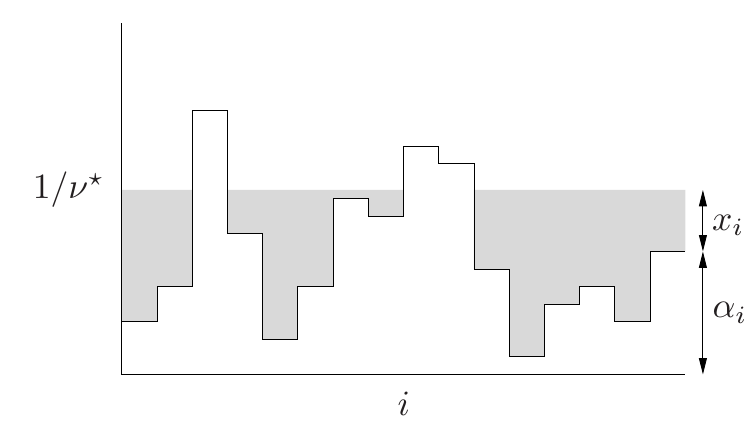
\includegraphics[width=0.7\textwidth]{assets/4 Duality/4.5 KKT optimality conditions/Water-filling solution.png}
  \caption{Water-filling solution}
\end{figure}

\subsection{Relationship with first-order conditions}
For a problem
\begin{align*}
\min \; &f_0(x)\\
\text{s.t.} \; &x \geq 0,
\end{align*}
the first-order condition is
\[
\nabla f_0(x^*) \succeq 0, \; x^* \succeq 0, \; x_i^* \nabla f_0(x^*)_i = 0, \; i = 1, 2, \ldots, n.
\]
The KKT condition is
\[
\nabla f_0(x^*) - \lambda^* = 0, \; x^* \succeq 0, \; \lambda^* \succeq 0, \; x_i^* \lambda_i^* = 0, \; i = 1, 2, \ldots, n.
\]
From the stationarity condition, we have $\lambda^* = \nabla f_0(x^*)$. Hence, the KKT condition is
equivalent to the first-order condition in this case.

Actually, the KKT condition is a generalization of the first-order condition when there are constraints.
For an unconstrained problem, the KKT condition is exactly the first-order condition.

\section{Sensitivity analysis}
\subsection{Perturbed problems}
Most of the time, the optimazation problem is perturbed by some parameters. For example, we have a
standard perturbed version of the problem
\begin{align*}
\min \; &f_0(x)\\
\text{s.t.} \; &f_i(x) \leq u_i, \; i = 1, 2, \ldots, m\\
&h_i(x) = w_i, \; i = 1, 2, \ldots, p.
\end{align*}
We define $p^*(u , w)$ as the optimal value of the perturbed problem. We have $p^*(0, 0) = p^*$.
The sensitivity analysis is to analyze how $p^*(u, w)$ changes with $u$ and $w$.

When the original problem is convex, $p^*(u, w)$ is a convex function. Here is the proof. We have
\begin{align*}
p^*(u, w) &= \inf_x \{f_0(x) \;|\; f_i(x) \leq u_i, i = 1, 2, \ldots, m; \; h_i(x) = w_i, i = 1, 2, \ldots, p\}\\
&= \inf_x g(x, u, w),
\end{align*}
where \[
g(x, u, w) = \begin{cases}
f_0(x), & f_i(x) \leq u_i, i = 1, 2, \ldots, m; \; h_i(x) = w_i, i = 1, 2, \ldots, p\\
+ \infty, & \text{otherwise}.
\end{cases}
\]
Obviously $g$ is convex. Hence, $p^*(u, w)$ is the pointwise infimum of a  convex function, which is
also convex.

\subsection{Global sensitivity}
Global sensitivity is defined that $\lambda^*, \nu^*$ is optimal for the original dual problem
if and only if the original problem is convex and strong duality holds. Written by
\[
p^*(u, w) \geq p^*(0, 0) - \lambda^{*T} u - \nu^{*T} w.
\]
This is much easy to understand. Assume $\tilde{x}$ is the optimal point of the perturbed problem.
We have
\begin{align*}
p^*(0, 0) &= g(\lambda^*, \nu^*)\\
&= \inf_x \{f_0(x) + \sum_{i=1}^m \lambda_i^* f_i(x) + \sum_{i=1}^p \nu_i^* h_i(x)\}\\
&\leq f_0(\tilde{x}) + \sum_{i=1}^m \lambda_i^* f_i(\tilde{x}) + \sum_{i=1}^p \nu_i^* h_i(\tilde{x})\\
&= p^*(u, w) + \lambda^{*T} u + \nu^{*T} w.
\end{align*}
And it's done.

According to these, we can conclude some cases.
\begin{itemize}
  \item To increase $p^*(u, w)$ greatly, we can let $\lambda^*$ be large and $u \preceq 0$
  or $\nu^*$ be large and positive and $w \preceq 0$ or $\nu^*$ be large and negative and $w \succeq 0$.
  \item To decrease $p^*(u, w)$ not much, we can let $\lambda^*$ be small and $u \succeq 0$
  or $\nu^*$ be small and positive and $w \succeq 0$ or $\nu^*$ be small and negative and $w \preceq 0$.
\end{itemize}

\subsection{Local sensitivity}
Suppose $p^*(u, w)$ is differentiable at $(0, 0)$. Then the local sensitivity is defined that
\[
\frac{\partial p^*(0, 0)}{\partial u_i} = - \lambda^*_i, \; \frac{\partial p^*(0, 0)}{\partial w_j} = - \nu^*_j.
\]
The proof will be omitted here. The local sensitivity tells us how active the constraints are.
For example, If $\lambda_i^*$ is large, the $i$-th constraint is active and we can increase $p^*(u, w)$
greatly by decreasing $u_i$. If $\lambda_i^*$ is small, the $i$-th constraint is inactive and we cannot
increase $p^*(u, w)$ much by decreasing $u_i$.

\section{Examples}
\subsection{Boolean LP problems}

Boolean LP problems are a special type of optimization problems where the decision variables are
restricted to be binary (0 or 1). These problems can be formulated as follows:
\begin{align*}
\min \; &c^T x\\
\text{s.t.} \; &Ax \leq b\\
&x \in \{0, 1\}, i = 1, 2, \ldots, n.
\end{align*}
It is much hard to solve because of the discrete nature. However, we can relax the problem by allowing
$x$ to take any value in the interval [0, 1], which can be formulated as
\begin{align*}
\min \; &c^T x\\
\text{s.t.} \; &Ax \leq b\\
&0 \leq x_i \leq 1, i = 1, 2, \ldots, n.
\end{align*}
The relaxed problem is a standard LP problem, which can be solved efficiently. The optimal value of
the relaxed problem provides a lower bound for the original Boolean LP problem. The dual problem of
it is
\begin{align*}
\max \; &-\lambda^T b - 1^T w\\
\text{s.t.} \; &c + A^T \lambda - \nu + w = 0\\
&\lambda \succeq 0, \; \nu \succeq 0, \; w \succeq 0.
\end{align*}
From these, we have $\nu_i = \max\{0, c_i + \lambda^T a_i\}$ and $w_i = -\min\{0, c_i + \lambda^T a_i\}$.
Hence, the dual problem can be rewritten as
\begin{align*}
\max \; &-\lambda^T b + 1^T w\\
\text{s.t.} \; &\lambda \succeq 0, \; w_i = \min\{0, c_i + \lambda^T a_i\}, i = 1, 2, \ldots, n.
\end{align*}

In the other way, if we don't want to relax it, we can reformulate the problem as
\begin{align*}
\min \; &c^T x\\
\text{s.t.} \; &Ax \leq b\\
&x_i (x_i - 1) = 0, i = 1, 2, \ldots, n.
\end{align*}
This is equivalent to the original problem. The reformulated problem is a nonconvex QCQP problem,
we can write its Lagrangian as
\[
L(x, \lambda, \nu) = \sum_{i=1}^n \nu_i x_i^2 + (c + \lambda^T A - \nu)^T x - \lambda^T b.
\]
Then the dual function is
\[
g(\lambda, \nu) = \begin{cases}
- \lambda^T b - \frac14 \sum_{i=1}^n \nu_i^{-1} (c_i + \lambda^T a_i - \nu_i)^2, & \nu \succ 0\\
+ \infty, & \text{otherwise}.
\end{cases}
\]
The dual problem is
\begin{align*}
\max \; &- \lambda^T b - \frac14 \sum_{i=1}^n \nu_i^{-1} (c_i + \lambda^T a_i - \nu_i)^2\\
\text{s.t.} \; &\lambda \succeq 0, \; \nu \succ 0.
\end{align*}
We have already known that
\[
\max_{x, y}f(x, y) = \max_x \max_y f(x, y),
\]
so we can analyze $\nu$ and $\lambda$ separately. For $\nu$, we have
\begin{align*}
\max_{\nu \succ 0} - \frac14 \sum_{i=1}^n \nu_i^{-1} (c_i + \lambda^T a_i - \nu_i)^2 &= \begin{cases}
0, & c_i + \lambda^T a_i > 0\\
c_i + \lambda^T a_i, & c_i + \lambda^T a_i \leq 0.
\end{cases}\\
&= \min\{0, c_i + \lambda^T a_i\}.
\end{align*}
And for $\lambda$, we have
\begin{align*}
\max_{\lambda} \; &-\lambda^T b + 1^T w\\
\text{s.t.} \; &\lambda \succeq 0, \; w_i = \min\{0, c_i + \lambda^T a_i\}, i = 1, 2, \ldots, n.
\end{align*}

The second method is called lagrangian relaxation. In this problem, two relaxations are the same.

\subsection{Quadratic penalty methods}

Consider a problem
\begin{align*}
\min \; &f_0(x)\\
\text{s.t.} \; &Ax = b,
\end{align*}
which $f_0(x)$ is convex and differentiable. We can change it to an unconstrained problem by adding a
penalty term to the objective function, which can be
\[
\min \; f_0(x) + \frac{\alpha}{2} ||Ax - b||_2^2.
\]
where $\alpha > 0$ is a penalty parameter. Let $\tilde{x}$ be the optimal point of the penalty problem.
We have
\begin{align*}
\tilde{x} &= \arg \min_x f_0(x) + \frac{\alpha}{2} ||Ax - b||_2^2.\\
&= \arg \min_x f_0(x) + \alpha (A \tilde{x} - b)^T (Ax - b),
\end{align*}
because the first-order condition of the two terms are both satisfied at $\tilde{x}$.

Now return to the original problem. The dual function is
\[
g(\nu) = \inf_x \{f_0(x) + \nu^T (Ax - b)\}.
\]
If we let $\nu = \alpha (A \tilde{x} - b)$, we have
\begin{align*}
g(\alpha (A \tilde{x} - b)) &= \inf_x \{f_0(x) + \alpha (A \tilde{x} - b)^T (Ax - b)\\
&= f_0(\tilde{x}) + \alpha||A \tilde{x} - b||_2^2
\end{align*}
From these we know
\[
f_0(x^*) = p^* \geq g(\alpha (A \tilde{x} - b)) = f_0(\tilde{x}) + \alpha||A \tilde{x} - b||_2^2 \geq f_0(\tilde{x}).
\]
In the end, we have $f_0(\tilde{x}) \to f_0(x^*)$ as $\alpha \to + \infty$.

\subsection{Log-barrier penalty methods}

Think about a problem
\begin{align*}
\min \; &f_0(x)\\
\text{s.t.} \; &Ax \geq b,
\end{align*}
we can change it to an unconstrained problem by adding a log-barrier penalty to the objective function,
which can be
\[
\min \; f_0(x) - \sum_{i=1}^m u_i \log(a_i^T x - b_i),
\]
where $u \succeq 0$ is a barrier parameter. Let $\tilde{x}$ be the optimal point of the penalty problem.
We have
\begin{align*}
\tilde{x} &= \arg \min_x f_0(x) - \sum_{i=1}^m u_i \log(a_i^T x - b_i) \\
&= \arg \min_x f_0(x) + \sum_{i=1}^m u_i \frac{a_i^T x - b_i}{a_i^T \tilde{x} - b_i}.
\end{align*}
The dual function of the original problem is
\[
g(\lambda) = \inf_x \{f_0(x) + \lambda^T (b - Ax)\}.
\]
If we let $\lambda_i = \frac{u_i}{a_i^T \tilde{x} - b_i}$, we have
\begin{align*}
g(\frac{u}{A \tilde{x} - b}) &= \inf_x \{f_0(x) + \sum_{i=1}^m u_i \frac{b_i - a_i^T x}{a_i^T \tilde{x} - b_i}\}\\
&= f_0(\tilde{x}) - \sum_{i=1}^m u_i \log(a_i^T \tilde{x} - b_i).
\end{align*}
From these we know
\[
f_0(x^*) = p^* \geq g(\frac{u}{A \tilde{x} - b}) = f_0(\tilde{x}) - \sum_{i=1}^m u_i \log(a_i^T \tilde{x} - b_i) \geq f_0(\tilde{x}).
\]
In the end, we have $f_0(\tilde{x}) \to f_0(x^*)$ as $u \to 0$. This method is called \textbf{interior
point method}, which is widely used in practice.

\newpage
\chapter{Unconstrained Minimization}
\section{Unconstrained minimization problems}
\subsection{Definition}
In this section we mainly talk about unconstrained minimization problems, which can be formulated as
\[
\min_x f(x),
\]
where $f(x)$ is a twice differentiable and convex function.

A necessary and sufficient condition for $x^*$ to be the optimal point is
\[
\nabla f(x^*) = 0.
\]
Thus, solving unconstrained minimization problems is equivalent to solving $\nabla f(x) = 0$.

\subsection{Strong convexity}
We say a function $f$ is strongly convex with parameter $m > 0$ if
\[
\nabla^2 f(x) \succeq m I, \; \forall x \in \textbf{dom } f.
\]
Such function has some nice properties. For example
\[
f(y) \geq f(x) + \nabla f(x)^T (y - x) + \frac{m}{2} |y - x|_2^2, \; \forall x, y \in \textbf{dom } f.
\]
Let $\tilde{y} = x- \frac{1}{m} \nabla f(x)$, we have
\[
f(y) \geq f(x) - \frac{1}{2m} ||\nabla f(x)||_2^2
\]
for all $y \in \textbf{dom } f$. This means that
\[
p^* \geq f(x) - \frac{1}{2m} ||\nabla f(x)||_2^2.
\]

We can also derive a bound on the distance between $x$ and $x^*$. We have
\[
||x - x^*||_2 \leq \frac{2}{m} ||\nabla f(x)||_2.
\]
To see this, let $y=x^*$, we have
\begin{align*}
  f(x^*) &\geq f(x) + \nabla f(x)^T (x^* - x) + \frac{m}{2} ||x^* - x||_2^2\\
  &\geq f(x) - ||\nabla f(x)||_2 ||x^* - x||_2 + \frac{m}{2} ||x^* - x||_2^2,
\end{align*}
where we use Cauchy-Schwarz inequality in the second inequality. Rearranging the terms, we have
\[
\frac{m}{2} ||x^* - x||_2^2 - ||\nabla f(x)||_2 ||x^* - x||_2 \leq 0.
\]
The solution is
\[
||x^* - x||_2 \leq \frac{2}{m} ||\nabla f(x)||_2.
\]

Moreover, $m$ is not the bigger the better. If $m \gg 0$, the function is too steep and the optimization
problem is sometimes hard to solve. So we often define the upper bound of the Hessian as $M$
and we have
\[
\nabla^2 f(x) \preceq M I, \; \forall x \in \textbf{dom } f.
\]
Just like the lower bound, we can also derive that
\[
f(y) \leq f(x) + \nabla f(x)^T (y - x) + \frac{M}{2} |y - x|_2^2, \; \forall x, y \in \textbf{dom } f.
\]
This leads to
\[
p^* \leq f(x) - \frac{1}{2M} ||\nabla f(x)||_2^2.
\]

\section{Descent method}
\subsection{Definition}
Descent method produces a minimizing sequence $x^k$ with $k = 0, 1, 2, \ldots$ which obeys
\begin{align*}
x^{k+1} &= x^k + t^k \Delta x^k\\
f(x^{k+1}) &< f(x^k).
\end{align*}
$\Delta x^k$ is called the search direction and $t^k$ is called the step size. The search direction
must satisfy
\[
\nabla f(x^k)^T \Delta x^k < 0,
\]
which means that $\Delta x^k$ is a descent direction. The step size can be determined by line search.

\subsection{Line search}
\subsubsection{Exact line search} the exact line search method chooses the step size $t$
to minimize $f(x^k + t \Delta x^k)$ with respect to $t$. This can be formulated as
\[
t = \argmin_{s > 0} f(x + s \Delta x).
\]
\subsubsection{Backtracking line search} the backtracking line search method chooses the step
size $t$ to satisfy the \textbf{Armijo condition}:
\[
f(x_k + t d_k) \leq f(x_k) + c t \nabla f(x_k)^T d_k,
\]
where $d_k$ is the descent direction and $c \in (0, 1)$.

\section{Gradient descent method}
\subsection{Definition}
At a point $x$, $-\nabla f(x)$ points in the direction where $f$ decreases the fastest. So at each step, we move
a bit in that direction:
\begin{equation}
x_{k+1} = x_k - t_k \nabla f(x_k),
\end{equation}
where $t_k > 0$ is called the step size. We stop when $||\nabla f(x_k)||_2 \leq \epsilon$
for some small tolerance $\epsilon > 0$.

\subsection{Step size}
\subsubsection{Fixed step size} Just set $t_k = t$ for all $k$. If $f$ satisfies
$m I \preceq \nabla^2 f(x) \preceq M I$, a popular pick in practice is $t = 2/(m + M)$. Howeever,
this requires knowing $m$ and $M$, which is often not available.

\subsubsection{Exact line search} At each step, solve
\[
t_k = \argmin_{t > 0} f(x_k - t \nabla f(x_k)).
\]
This gives the best possible decrease along the current direction. For quadratics
there is a closed form. But for general $f$, solving this subproblem exactly is
more expensive than the gradient step itself. So the next method is invented.

\subsubsection{Backtracking line search} Start with $t = 1$ and shrink it by a factor
$\beta \in (0, 1)$ until the Armijo condition holds:
\[
f(x_k - t \nabla f(x_k)) \leq f(x_k) - \alpha t ||\nabla f(x_k)||_2^2,
\]
where $\alpha \in (0, 0.5)$. This method is quite robust.

\subsection{Convergence analysis}
Define $\tilde{f}(x) = f(x - t \nabla f(x))$. Then we have
\[
\tilde{f}(t) \leq f(x) - t||\nabla f(x)||_2^2 + \frac{Mt^2}{2} ||\nabla f(x)||_2^2.
\]

\subsubsection{Exact line search} Differentiate the right-hand side with respect to $t$ and set it to
zero, we have $t = 1/M$. Then the problem becomes
\[
\min_t \tilde{f}(t) \leq f(x) - \frac{1}{2M} ||\nabla f(x)||_2^2,
\]
or rearranging it to
\[
f(x^{k+1}) \leq f(x^k) - \frac{1}{2M} ||\nabla f(x^k)||_2^2.
\]
This is called the \textbf{descent lemma}. It shows that the function value decreases at each step.
Beside this, we also have known that
\[
p^* \geq f(x^k) - \frac{1}{2m} ||\nabla f(x^k)||_2^2.
\]
Combining these two inequalities, we get
\[
\frac{f(x^{k+1}) - p^*}{f(x^k) - p^*} \leq (1 - \frac{m}{M}).
\]

Thus, if we want to find a point $x$ such that $\frac{f(x^{k+\tau}-p^*)}{f(x^k)-p^*} < \epsilon$,
we need at most $\tau = \frac{\log \epsilon}{\log (1 - m/M)}$ iterations.

\subsubsection{Backtracking line search} Set $t \in (0, \frac{1}{M})$, we have
\[
-t + \frac{Mt^2}{2} < -\frac{t}{2}.
\]
Using this, we have
\begin{align*}
\tilde{f}(t) &\leq f(x) - \frac{t}{2} ||\nabla f(x)||_2^2.\\
&\leq f(x) - \alpha t||\nabla f(x)||_2^2,
\end{align*}
where $\alpha <0.5$ according to the Armijo condition. This suggests that we know either $t = 1$
or $t \geq \frac{\beta}{M}$. Putting them together, we have
\[
f(x^{k+1}) \leq f(x) - \min\{\alpha, \frac{\beta \alpha}{M}\} ||\nabla f(x)||_2^2.
\]
And the final convergence rate is
\[
\frac{f(x^{k+1}) - p^*}{f(x^k) - p^*} = 1 - \min\{ 2m \alpha, \frac{2m \beta \alpha}{M} \}
\]

\section{Steepest descent method}
\subsection{Definition}
The first Taylor approximation of $f(x + v)$ at $x$ is
\[
f(x + v) \approx f(x) + \nabla f(x)^T v.
\]
The steepest descent method chooses the direction $v$ when $\nabla f(x)^T v < 0$. Also, we define
a normalized steepest descent direction as
\[
\Delta x_{nsd} = \argmin_{||v|| = 1} \nabla f(x)^T v.
\]
Next, to solve this problem, we should use line search.

\subsection{Variants}
\subsubsection{Euclidean norm} If we choose the Euclidean norm of $v$, the steepest descent method
is the same as the gradient descent method.

\subsubsection{$\ell_1$ norm} If we choose the $\ell_1$ norm of $v$, Because of the geometry of
the $\ell_1$ norm, we will have
\[
\Delta x_{nsd} = - \text{sign}(\nabla f(x))_i e_i,
\]
where $i = \arg \max_j |\nabla f(x)_j|$. This means that we only change the variable with the largest
gradient.

\subsubsection{Subgradient} There are some cases that $f$ is not differentiable. In this case,
we can use subgradient instead of gradients. Subgradient is defined as
\[
f(y) \geq f(x) + \partial f(x)^T (y - x), \; \forall y \in \textbf{dom } f,
\]
where $\partial f(x)$ is a subgradient of $f$ at $x$. Normally, subgradient is equal to gradient when $f$ is
differentiable, and be $[df(x_l), df(x_r)]$ when $f$ is not differentiable at $x$, where
$df(x_l)$ and $df(x_r)$ are the left and right derivatives of $f$. When $0 \in \partial f(x)$,
we have $x$ is the optimal point of $f$.

\section{Newton's method}
\subsection{Definition}
We call
\[
\Delta x_{nt} = -(\nabla^2 f(x))^{-1} \nabla f(x)
\]
the Newton step. And
\[
\lambda(x) = (\nabla f(x)^T \nabla^2 f(x)^{-1} \nabla f(x))^{1/2}
\]
the Newton decrement.

A simple (damped or guarded) Newton's method is as follows:
\begin{algorithm}[H]
\caption{Newton's method}
\begin{algorithmic}[1]
\State Choose $x \in \textbf{dom } f$ and $\epsilon > 0$.
\While{$\lambda(x)^2/2 > \epsilon$}
\State Compute the Newton step $\Delta x_{nt}$ and the Newton decrement $\lambda(x)$.
\State Choose the step size $t$ by backtracking line search.
\State Update $x = x + t \Delta x_{nt}$.
\EndWhile
\end{algorithmic}
\end{algorithm}

\subsection{Convergence analysis}
The convergence analysis of Newton's method is quite complex. We will only give a brief overview here.
For a $\eta > 0$, the convergence analysis of Newton's method can be divided into two phases.

\subsubsection{Phase 1: $\||\nabla f(x)||_2 \geq \eta$} In this phase, we called it the damped Newton phase.
The convergence rate is linear.

\subsubsection{Phase 2: $\||\nabla f(x)||_2 < \eta$} In this phase, we called it the quadratic
convergence phase. In this phase we often have
\[
\frac{f(x^{k+1}) - p^*}{{(f(x^k) - p^*)}^2} \approx c,
\]
where $c \in (0, 1)$ is a constant.

\newpage
\chapter{Equality Constrained Minimization}
\section{Equality constrained minimization problems}
\subsection{Definition}
Problems with equality constraints can be formulated as
\begin{align*}
\min \; &f(x)\\
\text{s.t.} \; &Ax = b,
\end{align*}
where $f(x)$ is a convex and twice differentiable function. Its KKT conditions are
\begin{align*}
\nabla f(x^*) + A^T \nu^* &= 0\\
Ax^* &= b.
\end{align*}
Solving equality constrained minimization problems is equivalent to solving the KKT conditions.

If $f(x)$ is quadratic, we can write it as
\[
f(x) = \frac12 x^T P x + q^T x + r,
\]
where $P \succeq 0$. Then the KKT conditions can be written as
\[
\begin{bmatrix}
  P & A^T \\
  A & 0
\end{bmatrix}
\begin{bmatrix}
  x^* \\ v^*
\end{bmatrix} =
\begin{bmatrix}
  -q \\ b
\end{bmatrix}.
\]
To solve this system, we can get the result of the original problem.

\subsection{Newton's method with equality constraints}
However, most of the time $f(x)$ is more complex. We can use Newton's method to solve it.
First we change the problem to such a form
\begin{align*}
\min \; &f(x^k + d)\\
\text{s.t.} \; &A(x^k + d) = b\\
&Ad = 0.
\end{align*}
To implement Newton's method, we can use the second-order Taylor approximation of $f(x^k + d)$:
\begin{align*}
\min \; &f(x^k) + \nabla f(x^k)^T d + \frac12 d^T \nabla^2 f(x^k) d\\
\text{s.t.} \; &Ad = 0,
\end{align*}
where $d^k = \argmin_d \{f(x^k) + \nabla f(x^k)^T d + \frac12 d^T \nabla^2 f(x^k) d\}$.
The KKT conditions of this problem are
\[
\begin{bmatrix}
  \nabla^2 f(x^k) & A^T \\
  A & 0
\end{bmatrix}
\begin{bmatrix}
  d^k \\ v^*
\end{bmatrix} =
\begin{bmatrix}
  -\nabla f(x^k) \\ 0
\end{bmatrix}.
\]
After solving $d^k$, we can update $x^{k+1} = x^k - t^k d^k$, where $t^k$ is the step size.
The step size can be determined by line search.

\section{Alternating Direction Method of Multipliers}
\subsection{Argumented Lagrangian Multiplier}

Let's start from a constrained optimization problem:
\[
  \min_x f(x), \quad s.t. \quad h(x) = 0
\]

We can form a Lagrangian function:
\[
  L(x, y) = f(x) + y^T (Ax - b)
\]

The origin problem is equivalent to the saddle point of $L(x, y)$. Usually we can
solve it by Lagrange dual ascent method:
\begin{algorithm}[H]
\caption{Lagrange Dual Ascent Method}
\begin{algorithmic}
\State Initialize $x^0$, $y^0$
\While{not converged}
  \State $x^{k+1} \gets \argmin_x L(x, y^k)$
  \State $y^{k+1} \gets y^k + \alpha (A x^{k+1} - b)$
\EndWhile
\State \Return $x^*$
\end{algorithmic}
\end{algorithm}

This method requires $f(x)$ to be strictly convex and differentiable. That means
we can't solve problems with non-smooth terms like $l_1$-norm or TV regularization.
To solve this problem, we can use Argumented Lagrangian Multiplier (ALM) method.

ALM adds a quadratic penalty term to the Lagrangian function:
\[
  L_\rho(x, y) = f(x) + y^T (Ax - b) + \frac{\rho}{2} ||Ax - b||_2^2
\]

This penalty term makes the function strongly convex, which helps to stabilize the
optimization process. The ALM method is similar to the dual ascent method:
\begin{algorithm}[H]
\caption{Augmented Lagrangian Multiplier}
\begin{algorithmic}
\State Initialize $x^0$, $y^0$
\While{not converged}
  \State $x^{k+1} \gets \argmin_x L_\rho(x, y^k)$
  \State $y^{k+1} \gets y^k + \rho (A x^{k+1} - b)$
\EndWhile
\State \Return $x^*$
\end{algorithmic}
\end{algorithm}

ALM directly uses $\rho$, which means higher numerical stability. However, $f(x)$
and $A$ will be quite complex in some cases, which makes step 2 hard to solve.
This is where Alternating Direction Method of Multipliers (ADMM) comes in.

\subsection{Alternating Direction Method of Multipliers}

Alternating Direction Method of Multipliers (ADMM) solves problems in the form of:
\[
  \min_{x,z} f(x) + g(z), \quad s.t. \quad Ax + Bz = c
\]

Now set ALM for this problem:
\[
  L_\rho(x, z, y) = f(x) + g(z) + y^T (Ax + Bz - c) + \frac{\rho}{2}
  ||Ax + Bz - c||_2^2
\]

If we optimize $x$ and $z$ together, it may be quite hard as the origin problem.
So ADMM optimizes $x$ and $z$ alternately, called \textbf{Gauss-Seidel} method:
\begin{algorithm}[H]
\caption{Alternating Direction Method of Multipliers}
\begin{algorithmic}
\State Initialize $x^0$, $z^0$, $y^0$
\While{not converged}
  \State $x^{k+1} \gets \argmin_x \left[ f(x) + \frac{\rho}{2} ||Ax + Bz^k - c + \frac{y^k}{\rho}||_2^2 \right]$
  \State $z^{k+1} \gets \argmin_z \left[ g(z) + \frac{\rho}{2} ||Ax^{k+1} + Bz - c + \frac{y^k}{\rho}||_2^2 \right]$
  \State $y^{k+1} \gets y^k + \rho (Ax^{k+1} + Bz^{k+1} - c)$
\EndWhile
\State \Return $x^*$, $z^*$
\end{algorithmic}
\end{algorithm}

In short, ADMM is a framwork to improve the efficiency of ALM. It is especially
useful when $f(x)$ and $g(z)$ are separable, which means they can be optimized
independently. This is often the case in practice, especially when $f(x)$ and
$g(z)$ are convex functions.

When facing a huge, complex and separable problem, ADMM is a good choice.
For example, Compressed Sensing, TV regularization, distributed optimization, etc.

\newpage
\chapter{Advanced Optimization Algorithms}
\section{Basic tools}
\subsection{Lipschitz}
A differentiable function $f$ is said to have an $L$-Lipschitz continuous gradient or
\textbf{$L$-smooth} if there exists a constant $L > 0$ such that
\[
\nabla f(x) - \nabla f(y) \leq L ||x - y||_2, \; \forall x, y \in \textbf{dom } f.
\]
Geometrically, this means that the gradient of $f$ does not change too rapidly.
The most important property of $L$-smooth functions is \textbf{descent lemma}, which have been
proved in the previous section. Here we give a more general form of the descent lemma:
\[
f(y) \le f(x) + \nabla f(x)^T (y-x) + \frac{L}{2} \|y-x\|_2^2.
\]
This is a quadratic upper bound on $f$. It suggests that $f$ cannot grow faster than a
quadratic function. This property is usually used to prove the convergence of optimization algorithms.

There are 2 main problems of Lipschitz functions. The first one is how to find the Lipschitz
constant $L$. The second one is what can we do if $f$ is not differentiable.

For the first problem, we can use the Hessian of $f$ to find $L$. If $f$ is twice differentiable,
we can use the following inequality:
\[
L \geq \sup_{x \in \textbf{dom } f} ||\nabla^2 f(x)||_2.
\]
There are also some other methods to find $L$. For example, if $f$ is a quadratic function, we can
use the largest eigenvalue of the Hessian matrix as $L$. If $f$ is a sum of functions, we can use the
largest Lipschitz constant of the functions as $L$. If $f$ is a composition of functions, we can use
the chain rule to find $L$. Besides these, we have power iteration method, we will talk about it later.

For the second problem, what we need is the concept of \textbf{proximal operator}.

\subsection{Proximal operator}
For a convex function $h: \mathbb{R}^n \to \mathbb{R} \cup \{+\infty\}$, its proximal operator is defined as
\[
\mathbf{prox}_h(v) = \argmin_{x} \left\{ h(x) + \frac{1}{2} \|x - v\|_2^2 \right\}.
\]
It may look intimidating at first, but the intuition is actually quite simple. Given a point $v$,
we want to find a new point $x$ that is both close to $v$ and makes the non-smooth function $h$ small.
The proximal operator strikes a balance between these two competing goals.

Proximal operators is much useful that it often has close-form solutions for many common non-smooth
functions. For example, the proximal operator of the $\ell_1$ norm is the soft-thresholding operator,
which is defined as
\[
[\mathbf{prox}_{\lambda \|\cdot\|_1}(v)]_i = \operatorname{sign}(v_i) \max\{|v_i| - \lambda, 0\}.
\]
This operator takes every component of $v$, shrinks it towards 0 by $\lambda$, and sets it to 0 if it
is smaller than $\lambda$. This is exactly why $\ell_1$ regularization promotes sparsity: small
coefficients are killed off entirely.

For most of the non-differentiable functions, we split them into a sum of a smooth part and a
non-smooth part. Then we can use Lipschitz and proximal operator to solve the problem separately.
This is the basic idea of many algorithms, such as  ADMM, FISTA, etc.

\subsection{Power iteration method}
The power iteration method is a simple and efficient algorithm for finding the largest eigenvalue
and corresponding eigenvector of a matrix. It is based on the idea that if we repeatedly multiply
a vector by a matrix, the direction of the vector will converge to the eigenvector corresponding
to the largest eigenvalue.

Given a matrix $A \in \mathbb{R}^{n \times n}$, the power iteration method proceeds as follows:
\begin{algorithm}[H]
\caption{Power Iteration method}
\begin{algorithmic}
\State Initialize $v_0$ with $\|v_0\|_2 = 1$.
\While{not converged}
  \State $w_{k+1} \gets A v_k$
  \State $v_{k+1} \gets w_{k+1} / \|w_{k+1}\|_2$
  \State $\lambda_{k+1} \gets v_{k+1}^T A v_{k+1}$
\EndWhile
\State \Return $(\lambda_{k+1}, v_{k+1})$
\end{algorithmic}
\end{algorithm}

The convergence behavior is quite elegant. Suppose the eigenvalues of $A$ are ordered as
\[
|\lambda_1| > |\lambda_2| \ge |\lambda_3| \ge \cdots \ge |\lambda_n|.
\]
Then the sequence $v_k$ converges to the eigenvector corresponding to $\lambda_1$ at a linear rate
proportional to $|\lambda_2 / \lambda_1|^k$. The closer $|\lambda_2|$ is to $|\lambda_1|$, the slower
the convergence. If $|\lambda_1| = |\lambda_2|$, the method may fail to converge.

You might be wondering: we are studying optimization, not linear algebra. Why do we need power iteration?
The answer is that many optimization algorithms require us to estimate the Lipschitz constant $L$ of a
quadratic function $f(x) = \frac12 x^T P x + q^T x + r$. As we mentioned in the Lipschitz subsection,
$L = \lambda_{\max}(P)$. When $n$ is large, computing all eigenvalues is a waste of time. Instead,
we can use power iteration to approximate $\lambda_{\max}(P)$ efficiently. We don't need the exact $L$;
a reasonably good upper bound is enough to set a safe step size.

There are a few things to keep in mind when using power iteration. First, the initial vector $v_0$
should not be orthogonal to the dominant eigenvector; otherwise, the method may converge to a
different eigenvector. In practice, choosing a random vector usually avoids this issue. Second,
if $A$ is not symmetric, the method still works for the largest singular value, but the eigenvalue
estimate $\lambda_{k+1} = v_{k+1}^T A v_{k+1}$ no longer gives the eigenvalue directly. For our
purposes, we will assume $A$ is symmetric, which is the case for Hessian matrices.

\section{Accelerated first-order methods}
\subsection{Fast gradient projection method}
We now arrive at our first advanced algorithm. The \textbf{Fast Gradient Projection} (FGP) method
is designed for problems of the form
\[
\min_{x \in \mathcal{C}} f(x),
\]
where $f$ is a smooth convex function with an $L$-Lipschitz continuous gradient, and $\mathcal{C}$
is a simple closed convex set onto which projection is computationally cheap. The projection
part comes from the fact that after taking a gradient step, we project the result back onto
$\mathcal{C}$ to enforce the constraint.

The basic \textbf{Gradient Projection} (GP) method is straightforward:
\[
x_{k+1} = P_{\mathcal{C}}\bigl( x_k - t_k \nabla f(x_k) \bigr),
\]
where $P_{\mathcal{C}}$ is the Euclidean projection onto $\mathcal{C}$ and $t_k$ is a step size
(often chosen as $1/L$ or via backtracking). This is essentially gradient descent with a projection
step.

FGP is the accelerated version. It incorporates Nesterov's momentum technique, which uses a cleverly
chosen extrapolation point $y_k$ to accelerate convergence. The algorithm is as follows:

\begin{algorithm}[H]
\caption{Fast Gradient Projection Method}
\begin{algorithmic}
\State Choose $x_0 \in \mathcal{C}$, set $y_1 = x_0$, $t_1 = 1$.
\For{$k = 1, 2, \ldots$}
  \State $x_k = P_{\mathcal{C}}\bigl( y_k - \frac{1}{L} \nabla f(y_k) \bigr)$
  \State $t_{k+1} = \frac{1 + \sqrt{1 + 4t_k^2}}{2}$
  \State $y_{k+1} = x_k + \frac{t_k - 1}{t_{k+1}} (x_k - x_{k-1})$ \quad (with $x_0 = x_{-1}$ for $k=1$)
\EndFor
\end{algorithmic}
\end{algorithm}

The sequence $x_k$ is the sequence of feasible points, while $y_k$ is the extrapolated point used
to compute the next gradient. The momentum term $(t_k-1)/t_{k+1}$ controls how much ``inertia''
from the previous step is carried over.

You might be wondering: what is this mysterious momentum term doing, and why does the sequence $t_k$
follow that peculiar recurrence with a square root?

In ordinary gradient descent, you compute the gradient at your current position $x_k$ and move
downhill. But by the time you get to the new point, the terrain may have changed direction.
Nesterov's trick is to first extrapolate where you are likely to be based on past momentum, then
compute the gradient at that extrapolated point, and finally step from there. This is why we
introduce the auxiliary sequence $y_k$. Think of $y_k$ as a ``prediction'' of where $x_k$ will be.
We take the gradient at $y_k$, not at $x_{k-1}$. Then we project and obtain $x_k$. After that,
we use the momentum term to update $y_{k+1}$ for the next iteration.

Now, what about that recurrence $t_{k+1} = \frac{1 + \sqrt{1 + 4t_k^2}}{2}$? It is not some arbitrary
trick. It is the precise mathematical formula that guarantees the optimal convergence rate. The role
of $t_k$ is to control the momentum coefficient $\frac{t_k - 1}{t_{k+1}}$. This coefficient starts
at $0$ and gradually increases towards $1$ as $k$ grows.

The remarkable property of FGP is its convergence rate. Under the same assumptions as gradient
descent, FGP achieves
\[
f(x_k) - f(x^*) \le \frac{2L \|x_0 - x^*\|_2^2}{(k+1)^2},
\]
which is $O(1/k^2)$—a significant improvement over the $O(1/k)$ rate of ordinary gradient projection.
This acceleration comes almost for free: each iteration still requires only one gradient evaluation
and one projection, just like the basic method. The only extra cost is a few vector operations to
compute the momentum.

Notice that if $\mathcal{C} = \mathbb{R}^n$, the projection is the identity map, and FGP reduces to
the well-known FISTA algorithm, which we will discuss later.

\subsection{Fast iterative shrinkage-thresholding algorithm}

Interative shrinkage-thresholding algorithm (ISTA) is designed for problems of the form
\[
\min_{x} \; f(x) = g(x) + h(x),
\]
where $g$ is smooth convex with an $L$-Lipschitz continuous gradient, and $h$ is convex but non-smooth.

ISTA applies the proximal operator of $h$ after each gradient step:
\[
x_{k+1} = \mathbf{prox}_{t h}\bigl( x_k - t \nabla g(x_k) \bigr).
\]
When $h(x) = \lambda \|x\|_1$, this becomes:
\[
x_{k+1} = \operatorname{soft}_{\lambda t}\bigl( x_k - t \nabla g(x_k) \bigr),
\]
where $\operatorname{soft}_{\lambda t}(\cdot)$ is the soft-thresholding operator. It means that
\[
[\operatorname{soft}_{\lambda t}(v)]_i = \operatorname{sign}(v_i) \max\{|v_i| - \lambda t, 0\}.
\]

ISTA converges at a rate of $O(1/k)$:
\[
f(x_k) - f(x^*) \le \frac{L \|x_0 - x^*\|_2^2}{2k}.
\]
This is the same as ordinary gradient descent. It works, but it is slow.

Fast iterative shrinkage-thresholding algorithm (FISTA) is the accelerated version of ISTA. The
algorithm is as follows:

\begin{algorithm}[H]
\caption{Fast Iterative Shrinkage-Thresholding Algorithm}
\begin{algorithmic}
\State Choose $x_0$, set $y_1 = x_0$, $t_1 = 1$.
\For{$k = 1, 2, \ldots$}
  \State $x_k = \operatorname{soft}_{\lambda/L}\bigl( y_k - \frac{1}{L} \nabla g(y_k) \bigr)$
  \State $t_{k+1} = \frac{1 + \sqrt{1 + 4t_k^2}}{2}$
  \State $y_{k+1} = x_k + \frac{t_k - 1}{t_{k+1}} (x_k - x_{k-1})$
\EndFor
\end{algorithmic}
\end{algorithm}

This is similar, FISTA uses the same Nesterov's momentum technique as FGP.

FISTA achieves the rate
\[
f(x_k) - f(x^*) \le \frac{2L \|x_0 - x^*\|_2^2}{(k+1)^2},
\]
which is $O(1/k^2)$. This is why FISTA has become the default solver for a vast range of problems.
It can solve most of the problems that people encounter in practice, and keep the same covergence
rate as FGP.

Moreover, FGP and FISTA are just special cases of a more general framework called
\textbf{Forward-Backward Splitting}.

\subsection{Forward-backward splitting}

Consider the composite optimization problem
\[
\min_{x} \; f(x) = g(x) + h(x),
\]
where $g$ is smooth convex with an $L$-Lipschitz continuous gradient, and $h$ is convex but
non-smooth. The name ``Forward-Backward'' comes from how we handle each part:
\begin{itemize}
  \item \textbf{Forward step}: we take an explicit gradient step on the smooth part $g$
  (moving forward in the direction of descent).
  \item \textbf{Backward step}: we apply the implicit proximal operator of the non-smooth part $h$
  (which can be seen as a backward Euler step).
\end{itemize}

The iteration is strikingly simple:
\[
x_{k+1} = \mathbf{prox}_{t h}\bigl( x_k - t \nabla g(x_k) \bigr),
\]
where $t > 0$ is a step size (typically $t = 1/L$). 

Let us see how this framework unifies several well-known algorithms:
\begin{itemize}
  \item If $h(x) = I_{\mathcal{C}}(x)$ (the indicator function), then
  $\mathbf{prox}_{t h} = P_{\mathcal{C}}$, and FBS becomes the basic GP method.
  \item If $h(x) = \lambda \|x\|_1$, then $\mathbf{prox}_{t h}$ becomes the soft-thresholding
  operator, and FBS becomes ISTA.
\end{itemize}

In other words, FGP and FISTA are just FBS with different proximal operators. The difference
between projection and shrinkage is not a difference in algorithm design, but merely a
difference in which non-smooth function $h$ we choose.

Under the standard step size $t = 1/L$, FBS converges with rate $O(1/k)$:
\[
f(x_k) - f(x^*) \le \frac{L \|x_0 - x^*\|_2^2}{2k}.
\]
This is the same as ordinary gradient descent.

Understanding FBS gives you a powerful mental model: any problem of the form ``smooth + non-smooth''
can be solved by alternating a gradient step and a proximal step. The only thing that changes from
problem to problem is the closed-form expression of the proximal operator. Once you memorize the
proximal operators for $\ell_1$, $\ell_2$ squared, nuclear norm, and indicator functions, you
can instantly write down solvers for LASSO, ridge regression, matrix completion, and constrained
optimization.

\section{Nonlinear least squares problems}
\subsection{Gauss–Newton Method}

The Gauss–Newton method is the classical approach for nonlinear least squares. It exploits
the special structure of the objective: if $F(x)$ were linear, the problem would reduce to linear
least squares, which has a closed-form solution. The idea is to repeatedly linearize $F$ around
the current iterate and solve the resulting linear least squares subproblem.

At iteration $k$, we approximate $F$ by its first-order Taylor expansion around $x_k$:
\[
F(x_k + d) \approx F(x_k) + J(x_k) d,
\]
where $J(x_k) \in \mathbb{R}^{m \times n}$ is the Jacobian matrix of $F$ at $x_k$, which means
\[
J(x_k) = \begin{bmatrix}
  \nabla F_1(x_k)^T \\
  \nabla F_2(x_k)^T \\
  \vdots \\
  \nabla F_m(x_k)^T
\end{bmatrix}.
\]

We turn the problem into:
\[
F(x_k + d) \approx \frac12 \|F(x_k) + J(x_k) d\|_2^2.
\]
This is a linear least squares problem. Minimizing it gives the Gauss–Newton step:
\[
d_{GN} = \argmin_{d} \frac12 \|F(x_k) + J(x_k) d\|_2^2.
\]
The solution satisfies the normal equations:
\[
J(x_k)^T J(x_k) \, d_{GN} = -J(x_k)^T F(x_k).
\]
We then update $x_{k+1} = x_k + d_{GN}$.

If $F$ is nearly linear or if the residual $\|F(x)\|_2$ is small at the solution, Gauss–Newton
converges very quickly. This is because the Hessian of $f$ is approximately $J^T J$ when the
residual is small.

However, Gauss-Newton can fail if $J^T J$ is ill-conditioned. The normal equations cannot be
solved reliably, and the step $d_{GN}$ may become enormous or point in a completely wrong direction.
This happens frequently in practice — for example, when the parameters are poorly identifiable
or when the problem is overparameterized. Thanks to Levenberg and Marquardt, we have a simple fix
to stabilize the method.

\subsection{Levenberg–Marquardt Method}

The Levenberg–Marquardt method (L-M) is a simple but brilliant fix to the Gauss–Newton instability.
The idea is to add a damping term to the normal equations:
\[
(J^T J + \mu I) \, d = -J^T F,
\]
where $\mu > 0$ is a damping parameter. Instead of solving the original normal equations, we solve
this regularized system.

Why does this work? Let us examine two extreme cases:
\begin{itemize}
  \item If $\mu$ is very large, the term $\mu I$ dominates, and the step becomes approximately
  \[
  d \approx -\frac{1}{\mu} J^T F.
  \]
  This is exactly a steepest descent direction. It is guaranteed to decrease the objective,
  but convergence is slow.
  \item If $\mu$ is very small, the system reduces to the Gauss–Newton equations. The step inherits
  the fast local convergence of Gauss–Newton.
\end{itemize}

The magic of L-M is that it \textbf{interpolates between gradient descent and Gauss–Newton}.
When the step is working well, we decrease $\mu$ to move closer to Gauss–Newton and speed up
convergence. When the step fails, we increase $\mu$ to move closer to gradient descent and stabilize
the algorithm. This adaptive behavior makes L-M one of the most robust and widely used algorithms
for nonlinear least squares.

A typical L-M implementation proceeds as follows:

\begin{algorithm}[H]
\caption{Levenberg–Marquardt Method}
\begin{algorithmic}
\State Choose $x_0$, $\mu_0 > 0$, and parameters $\beta_{\text{inc}} > 1$, $\beta_{\text{dec}} \in (0, 1)$.
\For{$k = 0, 1, 2, \ldots$}
  \State Compute $F(x_k)$ and $J(x_k)$.
  \State Solve $(J^T J + \mu_k I) \, d_k = -J^T F$.
  \State Compute $x_{\text{new}} = x_k + d_k$.
  \State Compute the gain ratio:
  \[
  \rho = \frac{f(x_k) - f(x_{\text{new}})}{\frac12 d_k^T (\mu_k d_k - J^T F)}.
  \]
  \If{$\rho > 0$}
    \State Accept the step: $x_{k+1} = x_{\text{new}}$.
    \State Decrease the damping: $\mu_{k+1} = \mu_k \cdot \beta_{\text{dec}}$.
  \Else
    \State Reject the step: $x_{k+1} = x_k$.
    \State Increase the damping: $\mu_{k+1} = \mu_k \cdot \beta_{\text{inc}}$.
  \EndIf
\EndFor
\end{algorithmic}
\end{algorithm}

The gain ratio $\rho$ compares the actual reduction in $f$ to the reduction predicted by the linear
model. If $\rho$ is positive, the model is accurate and we decrease $\mu$. If $\rho$ is too small
or negative, the model is poor and we increase $\mu$ to take a more conservative step.

L-M converges globally if $\mu$ is managed correctly: when $\mu$ is large, the step is a descent
direction, so the objective decreases. As the iterate approaches a local minimum, $\mu$ typically
becomes small and the method exhibits the fast quadratic convergence of Gauss–Newton.

In practice, L-M is the go-to solver for small-to-medium scale nonlinear least squares problems.
It is the default algorithm in many optimization libraries. It requires solving a linear system
at each iteration, which costs $O(n^3)$ for dense problems, so it is not suitable for very large
$n$. But when accuracy matters and $n$ is modest, L-M is hard to beat.

\subsection{Quasi-Newton methods}
Quasi-Newton methods are a class of optimization algorithms that aim to achieve the fast convergence
of Newton's method without the computational burden of calculating and inverting the Hessian matrix.

Remember that Newton's method updates the iterate as
\[
x_{k+1} = x_k - H_k^{-1} \nabla f(x_k),
\]
where $H_k = \nabla^2 f(x_k)$ is the Hessian. Computing $H_k$ and its inverse can be expensive,
especially in high dimensions. Quasi-Newton methods approximate $H_k^{-1}$ using information from
previous iterations.

The most famous quasi-Newton method is the Broyden–Fletcher–Goldfarb–Shanno (BFGS) algorithm.
It maintains a positive definite matrix $B_k$ that approximates the inverse Hessian. Define
\[
s_k = x_{k+1} - x_k, \qquad y_k = \nabla f(x_{k+1}) - \nabla f(x_k).
\]
The update rule is:
\[
B_{k+1} = B_k - \frac{B_k s_k s_k^T B_k}{s_k^T B_k s_k} + \frac{y_k y_k^T}{y_k^T s_k}.
\]

This is a rank-2 update: we add two outer products to $B_k$, so the cost of each iteration
is $O(n^2)$ — far cheaper than the $O(n^3)$ required for computing and inverting the true Hessian.
The formula is designed so that:
\begin{itemize}
  \item $B_{k+1}$ satisfies the \textbf{secant condition}: $B_{k+1} y_k = s_k$.
  \item If $B_k$ is positive definite and $y_k^T s_k > 0$, then $B_{k+1}$ remains positive definite.
\end{itemize}

For large-scale problems, the limited-memory BFGS (L-BFGS) variant is often used. L-BFGS keeps only
the last $m$ pairs of $(s_k, y_k)$ to approximate the inverse Hessian. This reduces memory usage
from $O(n^2)$ to $O(mn)$.


\newpage
\appendix
\chapter{Quiz}
\section{Quiz 1}
Prove the geometric mean function
\[
f(x) = (\prod_{i = 1}^n x_i)^{1/n}, \; x \in \mathbb{R}
\]
is concave when $\textbf{dom } f = S = \mathbb{R}^n_{++} \cap \{ ||x||_2 \leq 1 \}$.

Note that we cannot directly use second-order conditions because $\textbf{dom } f$ is a
half-open interval, suggesting it's not twice differentiable.

What can we do? Remember in 2.1.4 we talked about the geometric mean function is concave
on $\mathbb{R}^n_{++}$. And $S$ is a convex set. The concavity is preserved on the convex
set.

\section{Quiz 2}
\subsection{Quiz 2.1}
Prove that
\begin{align*}
\max_{v, \lambda_1, \lambda_2}& -b^T v - \lambda_1^T u + \lambda_2^T l\\
\text{s.t.}& \; A^T v + \lambda_1 - \lambda_2 + c = 0\\
&\lambda_1 \succeq 0, \; \lambda_2 \succeq 0
\end{align*}
is equivalent to
\[
\max_{v} -b^T v - u^T (A^T v + c)^- + l^T (A^T v + c)^+.
\].

We can rewrite the problem as
\[
\max_{v} \left\{ 
    -b^T v +
    \underbrace{
        \max_{\substack{\lambda_1, \lambda_2 \succeq 0 \\ \lambda_2 - \lambda_1 = \omega}} \left( -\lambda_1^T u + \lambda_2^T l \right)
    }_{\text{Inner maximization problem}}
\right\}
\]
Let $\omega = A^T v + c$. Then we know
\[
\lambda_2 - \lambda_1 = \omega,
\]
then let $\lambda_1 = \alpha$ and $\lambda_2 = \alpha + \omega$, where $\alpha \succeq 0$. We have
\[
\alpha_i \geq \max(0, -\omega_i) = \omega_i^-.
\]
Now we can rewrite the inner maximization problem as
\[
\sum_i [-u_i \alpha_i + l_i (\alpha_i + \omega_i)] = \sum_i [(l_i - u_i) \omega_i + l_i \omega_i]
\]
when $a_i = \omega_i^-$. Also, according to $\omega_i = \omega_i^+ - \omega_i^-$, we can infer that
\[
(l_i - u_i) \omega_i + l_i \omega_i = l_i \omega_i^+ - u_i \omega_i^-.
\]
Till now the inner maximization problem is reformulated as
\[
-u^T \omega^- + l^T \omega^+.
\]
This is the same as $\max_v -u^T (A^T v + c)^- + l^T (A^T v + c)^+$.

\subsection{Quiz 2.2}
Prove that
\[
p(u, \omega)  = \inf_x g(x, u, \omega)
\]
is convex when $g(x, u, \omega)$ is convex.

Select $(\omega_1, u_1)$, $(\omega_2, u_2)$ and $\theta \in [0, 1]$, and
\[
(u_{\theta}, \omega_{\theta}) = \theta (u_1, \omega_1) + (1 - \theta) (u_2, \omega_2),
\]
what we need to prove is
\[
p(u_{\theta}, \omega_{\theta}) \leq \theta p(u_1, \omega_1) + (1 - \theta) p(u_2, \omega_2).
\]

We know
\begin{align*}
g(x_1, u_1, \omega_1) &\leq p(u_1, \omega_1) + \epsilon\\
g(x_2, u_2, \omega_2) &\leq p(u_2, \omega_2) + \epsilon
\end{align*}
for any $\epsilon > 0$.

Let $x_{\theta} = \theta x_1 + (1 - \theta) x_2$. Then we have
\begin{align*}
p(u_{\theta}, \omega_{\theta}) &\leq g(x_{\theta}, u_{\theta}, \omega_{\theta})\\
&\leq \theta g(x_1, u_1, \omega_1) + (1 - \theta) g(x_2, u_2, \omega_2)\\
&\leq \theta p(u_1, \omega_1) + (1 - \theta) p(u_2, \omega_2) + \epsilon.
\end{align*}
Since $\epsilon$ is arbitrary, we have
\[
p(u_{\theta}, \omega_{\theta}) \leq \theta p(u_1, \omega_1) + (1 - \theta) p(u_2, \omega_2)
\]
when $\epsilon \to 0$. Hence, $p(u, \omega)$ is convex.

\newpage
\chapter*{Afterword}
\addcontentsline{toc}{chapter}{Afterword}

I began this tutorial on Jan 11, 2026. I wrote about half of it during the winter vacation,
and then almost nothing until my summer vacation began. You are welcome to laugh at my laziness
— honestly, no one wants to write anything during the semester. But I am glad I finally finished it.

This tutorial was written mostly after my compressed sensing tutorial, so I have made a lot of
improvements since then. The typesetting is cleaner, the math formulas are more readable, and
I have learned (the hard way) not to define every theorem environment from scratch. The
ElegantBook template did most of the heavy lifting this time, and I am grateful for that.

Looking back, there are several topics I wish I could have covered. Interior-point methods,
which dominate commercial solvers, are barely mentioned. Robust optimization, semidefinite
programming applications, and non-convex heuristics are all worth entire chapters of their own.
Perhaps in a future version — or perhaps someone else will write those chapters.

\subsection*{What I learned from writing this}

Writing a tutorial forces you to confront what you do and do not understand. It is easy to read
a proof and nod along; it is much harder to explain it to someone else in plain language. Many
times I thought I understood a topic — only to discover, when I sat down to write about it,
that my understanding was superficial at best. Some sections took me far longer than I expected,
because I had to work through the derivations myself before I could write them down clearly.

If you are my junior reading this: try writing your own notes. Not bullet points — full sentences,
with proofs and code. You will be surprised how much you learn in the process.

\subsection*{A note on the cover}

The cover image is a TikZ drawing I made for this tutorial. It shows a convex function surface
drawn as contour ellipses, with several gradient descent paths zigzagging toward the minimum.
I wanted something that captured the spirit of the book: geometric intuition, iterative algorithms,
and the idea that from any starting point, you can eventually find your way down.

A piece of advice for those who are just starting out: do not be intimidated by the mathematical
notation. Convex optimization looks heavy on paper, but the core ideas are actually quite intuitive.
When you see a formula, try to draw it, visualize it, or implement it in MATLAB. Math is not that
frightening when you can see it in action. And if you are struggling with a concept, do not hesitate
to ask for help — the optimization community is one of the friendliest corners of applied mathematics.

Next, I plan to rewrite my compressed sensing tutorial into a digital image processing tutorial,
with compressed sensing as just one chapter in it. After that, who knows — maybe a tutorial on
numerical linear algebra, or maybe I will finally read Boyd's book cover to cover and update this
one. Life is short — study hard, play hard, and enjoy both.

\begin{flushright}
  Lancet Ross\\
  Jul 22, 2026
\end{flushright}

\end{document}